\documentclass[11pt,a4paper]{article}
\usepackage[utf8]{inputenc}
\usepackage[T1]{fontenc}
\usepackage{lmodern}
\usepackage{amsmath, amssymb, amsfonts}
\usepackage{graphicx}
\usepackage{booktabs}
\usepackage{geometry}
\usepackage{hyperref}
\usepackage{tcolorbox}
\usepackage{enumitem}
\usepackage{xcolor}
\usepackage{float}
\usepackage{longtable}
\usepackage{caption}

\geometry{margin=0.9in}
\hypersetup{
    colorlinks=true,
    linkcolor=blue,
    filecolor=magenta,
    urlcolor=cyan,
    pdftitle={NLTP Complete Study Material v2},
}

\setlist[itemize]{itemsep=0.5em, topsep=0.5em, parsep=0.2em}
\setlist[enumerate]{itemsep=0.5em, topsep=0.5em, parsep=0.2em}

\title{\textbf{Natural Language Processing and Text Processing (NLTP)\\Complete Study Material — Elaborated Edition}}
\author{Generated from course material with full theory and diagrams}
\date{}

\begin{document}

\maketitle
\tableofcontents
\newpage

\section{Module 1: N-gram Language Models and Edit Distance}

\subsection{Introduction to Language Models}

A \textbf{language model} is a fundamental component of many natural language processing systems. In its most basic form, a language model is a machine learning model that predicts upcoming words in a sequence. More formally, a language model assigns a probability to each possible next word, or equivalently, it defines a probability distribution over the entire vocabulary of possible next words given some preceding context. This probabilistic framework allows language models to quantify how likely a particular sequence of words is to occur in a language, which makes them useful for a wide range of applications including speech recognition, machine translation, spelling correction, and text generation.

The power of a language model lies in its ability to capture the statistical regularities of a language. For example, given the partial sentence ``The cat sat on the\_\_'', a good language model should assign a much higher probability to ``mat'' than to ``refrigerator'', because the former is far more likely in natural English. Language models can also assign a probability to an entire sentence, which is useful for ranking candidate outputs in tasks like machine translation or speech recognition, where multiple candidate sentences might be generated and the one with the highest probability according to the language model is preferred.

\textbf{Applications of language models} are extensive and form the backbone of many practical NLP systems:
\begin{itemize}
    \item \textbf{Spelling and grammar correction}: A language model can detect errors such as ``Their are'' (which should be ``There are'') by assigning a much lower probability to the incorrect sequence.
    \item \textbf{Speech recognition disambiguation}: When a speech recognizer is uncertain between acoustically similar words (e.g., ``recognize speech'' vs. ``wreck a nice beach''), a language model helps choose the more probable sequence.
    \item \textbf{Augmentative and Alternative Communication (AAC)}: Language models can predict the next word for users with disabilities, reducing the effort required to type or communicate.
    \item \textbf{Machine translation}: Language models score candidate translations to select the most fluent output.
\end{itemize}

\subsection{N-gram Language Models}

An \textbf{n-gram} is a contiguous sequence of $n$ items from a given text or speech. In the context of language modeling, these items are typically words, though they can also be characters or phonemes. The simplest n-grams are:
\begin{itemize}
    \item \textbf{Unigram} (1-gram): A single word, such as ``The''.
    \item \textbf{Bigram} (2-gram): A two-word sequence, such as ``The water''.
    \item \textbf{Trigram} (3-gram): A three-word sequence, such as ``The water of''.
\end{itemize}

An n-gram language model estimates the probability of a word based on the previous $n-1$ words. The most common types are unigram, bigram, and trigram models, though higher-order models (4-grams, 5-grams) are also used when sufficient training data is available. The choice of $n$ involves a trade-off: higher-order models capture more context and generally make better predictions, but they require exponentially more data to estimate reliably and become increasingly sparse (many possible n-grams never appear in the training data).

\subsubsection{Chain Rule of Probability}

The foundation of n-gram language modeling is the \textbf{chain rule of probability} (also called the product rule). The chain rule allows us to decompose the joint probability of a sequence of words into a product of conditional probabilities. For a sequence of words $w_1, w_2, \ldots, w_n$, the joint probability is:
\[
P(w_1, w_2, \ldots, w_n) = P(w_1) \times P(w_2 \mid w_1) \times P(w_3 \mid w_1, w_2) \times \cdots \times P(w_n \mid w_1, w_2, \ldots, w_{n-1})
\]
This equation is exact, but computing the conditional probability $P(w_n \mid w_1, \ldots, w_{n-1})$ requires knowing the probability of a word given its entire history, which is impractical because the number of possible histories grows exponentially with sentence length. This motivates the Markov assumption.

\subsubsection{The Markov Assumption}

The \textbf{Markov assumption} simplifies the chain rule by assuming that the probability of a word depends only on a finite window of preceding words, rather than the entire history. This is also called the \textbf{Markov property} or \textbf{limited horizon} assumption. Formally, for a bigram model, the probability of a word depends only on the immediately preceding word:
\[
P(w_n \mid w_1, w_2, \ldots, w_{n-1}) \approx P(w_n \mid w_{n-1})
\]

For a general n-gram model, the probability depends on the previous $N-1$ words:
\[
P(w_n \mid w_1, w_2, \ldots, w_{n-1}) \approx P(w_n \mid w_{n-N+1}, \ldots, w_{n-1})
\]

This assumption is clearly false in a strict sense---the meaning of a word often depends on words much earlier in the sentence. However, the Markov assumption makes language models computationally tractable and, in practice, bigram and trigram models capture enough local context to be surprisingly effective for many tasks.

\subsubsection{Maximum Likelihood Estimation (MLE)}

To estimate the conditional probabilities in an n-gram model, we use \textbf{Maximum Likelihood Estimation (MLE)}, which simply counts how often each n-gram occurs in a training corpus and normalizes these counts. For a bigram model, the MLE estimate is:
\[
P(w_n \mid w_{n-1}) = \frac{C(w_{n-1}, w_n)}{C(w_{n-1})}
\]
where $C(w_{n-1}, w_n)$ is the count of the bigram (the number of times the two-word sequence appears together in the training corpus), and $C(w_{n-1})$ is the count of the first word (the number of times the context word appears).

For a general n-gram, the MLE estimate is:
\[
P(w_n \mid w_{n-N+1}, \ldots, w_{n-1}) = \frac{C(w_{n-N+1}, \ldots, w_n)}{C(w_{n-N+1}, \ldots, w_{n-1})}
\]

This estimation method is straightforward but has a critical limitation: if a particular n-gram never appears in the training data, its MLE probability is zero, which can cause the entire sentence probability to collapse to zero.

\begin{tcolorbox}[colback=blue!5!white,colframe=blue!75!black,title=\textbf{Worked Example: Berkeley Restaurant Project Bigram Counts}]
Consider a mini-corpus with sentences augmented by start-of-sentence \texttt{<s>} and end-of-sentence \texttt{</s>} markers:
\begin{itemize}
    \item \texttt{<s> I am Sam </s>}
    \item \texttt{<s> Sam I am </s>}
    \item \texttt{<s> I do not like green eggs and ham </s>}
\end{itemize}

Sample bigram probability calculations using MLE:
\[
P(\text{I} \mid \text{<s>}) = \frac{2}{3} = 0.67, \quad
P(\text{Sam} \mid \text{<s>}) = \frac{1}{3} = 0.33
\]
\[
P(\text{am} \mid \text{I}) = \frac{2}{3} = 0.67, \quad
P(\text{do} \mid \text{I}) = \frac{1}{3} = 0.33
\]
\[
P(\text{</s>} \mid \text{Sam}) = \frac{1}{2} = 0.5, \quad
P(\text{Sam} \mid \text{am}) = \frac{1}{2} = 0.5
\]

The sentence probability is the product of all bigram probabilities along the path through the sentence. For example:
\[
P(\text{<s> I want english food </s>}) = P(\text{I}|\text{<s>}) \times P(\text{want}|\text{I}) \times P(\text{english}|\text{want}) \times P(\text{food}|\text{english}) \times P(\text{</s>}|\text{food})
\]
\end{tcolorbox}

\subsubsection{Log Probabilities}

Language model probabilities are typically stored and computed as \textbf{log probabilities} to avoid numerical underflow. When we multiply many small probabilities together (as we do when computing the probability of a long sentence), the product can become smaller than the smallest representable floating-point number, causing underflow to zero. By working in log space, multiplication becomes addition, which is both numerically stable and computationally faster:
\[
\log(p_1 \times p_2 \times p_3 \times p_4) = \log p_1 + \log p_2 + \log p_3 + \log p_4
\]
Since log is a monotonically increasing function, the word sequence with the highest probability also has the highest log probability, so we can safely work in log space without changing the ranking of candidate sequences.

\subsection{Evaluating Language Models}

Before we can use a language model, we must evaluate its quality. There are two primary approaches to evaluation: extrinsic and intrinsic. Understanding the distinction is important because different evaluation methods serve different purposes and have different costs.

\subsubsection{Training, Test, and Development Sets}

When building any machine learning model, we partition our data into distinct subsets to ensure unbiased evaluation:
\begin{itemize}
    \item \textbf{Training set}: The data used to learn the model parameters. For an n-gram model, this means counting n-gram frequencies and computing probabilities.
    \item \textbf{Test set}: A held-out portion of the data that the model has never seen during training. This gives an unbiased estimate of how the model will perform on new, unseen text.
    \item \textbf{Development set} (or validation set): An intermediate set used for tuning hyperparameters, trying different model variants, and making design decisions without contaminating the test set.
\end{itemize}

\textbf{Data contamination} occurs when the test set is used during training or when information from the test set leaks into the model development process. This leads to artificially optimistic performance estimates and models that fail to generalize to truly new data.

\subsubsection{Extrinsic vs. Intrinsic Evaluation}

\textbf{Extrinsic evaluation} embeds the language model in an end-to-end application and measures whether the application performs better. For example, we might compare two language models by measuring which one yields lower word error rate in a speech recognition system. While extrinsic evaluation is the ultimate measure of usefulness, it is expensive and time-consuming because it requires building and running the full application for every model variant.

\textbf{Intrinsic evaluation} measures the quality of the model independently of any specific application. The most common intrinsic metric for language models is \textbf{perplexity}, which is fast to compute and correlates reasonably well with extrinsic performance. Intrinsic evaluation allows researchers to compare many model variants quickly before selecting the best for extrinsic testing.

\subsubsection{Perplexity}

\textbf{Perplexity} (often abbreviated as PP or PPL) is the standard intrinsic evaluation metric for language models. Intuitively, perplexity measures how ``surprised'' the model is by the test data. A model that assigns high probabilities to the words that actually appear in the test set has low perplexity; a model that is frequently surprised by the test data has high perplexity.

Mathematically, perplexity is the inverse probability of the test set, normalized by the number of words $N$:
\[
\text{Perplexity}(W) = P(w_1, w_2, \ldots, w_N)^{-\frac{1}{N}}
\]

For a bigram model, using the chain rule, this becomes:
\[
\text{Perplexity}(W) = \sqrt[N]{\prod_{i=1}^{N} \frac{1}{P(w_i \mid w_{i-1})}}
\]

An important property of perplexity is that it can also be interpreted as the \textbf{weighted average branching factor} of the language. The branching factor is the number of possible next words that could follow any given word. For a language with vocabulary size $V$, the maximum perplexity is $V$ (uniform distribution), and the minimum is 1 (perfect prediction).

\begin{tcolorbox}[colback=green!5!white,colframe=green!75!black,title=\textbf{Numerical: Perplexity as Weighted Average Branching Factor}]
\textbf{Given}: A language $L = \{\text{red, blue, green}\}$ with branching factor 3.

\textbf{Model A}: Each word follows with equal probability $\frac{1}{3}$.
Test sequence: ``red red red red blue'' ($N=5$)
\[
\text{Perplexity}_A = \left(\frac{1}{3}\right)^{-\frac{5}{5}} = \left(\frac{1}{3}\right)^{-1} = 3
\]

\textbf{Model B}: $P(\text{red}) = 0.8$, $P(\text{green}) = 0.1$, $P(\text{blue}) = 0.1$
\[
P(\text{red red red red blue}) = 0.8^4 \times 0.1 = 0.04096
\]
\[
\text{Perplexity}_B = (0.04096)^{-\frac{1}{5}} = 0.527^{-1} = 1.89
\]

\textbf{Interpretation}: Although both models have the same branching factor (3 possible next words), Model B has lower perplexity because it predicts ``red'' correctly most of the time. The probabilities assigned by the model directly determine how surprised it is by the test data.
\end{tcolorbox}

\begin{tcolorbox}[colback=green!5!white,colframe=green!75!black,title=\textbf{Numerical: Perplexity on WSJ Corpus}]
The table below shows perplexity values for unigram, bigram, and trigram models trained on 38 million words from the Wall Street Journal, evaluated on a 1.5 million word test set:
\begin{center}
\begin{tabular}{|c|c|c|}
\hline
\textbf{Unigram} & \textbf{Bigram} & \textbf{Trigram} \\ \hline
962 & 170 & 109 \\ \hline
\end{tabular}
\end{center}

As expected, higher-order models (which incorporate more context) assign higher probabilities to the test data and therefore achieve lower perplexity. The trigram model is nearly 9 times better than the unigram model by this metric.
\end{tcolorbox}

\begin{figure}[H]
    \centering
    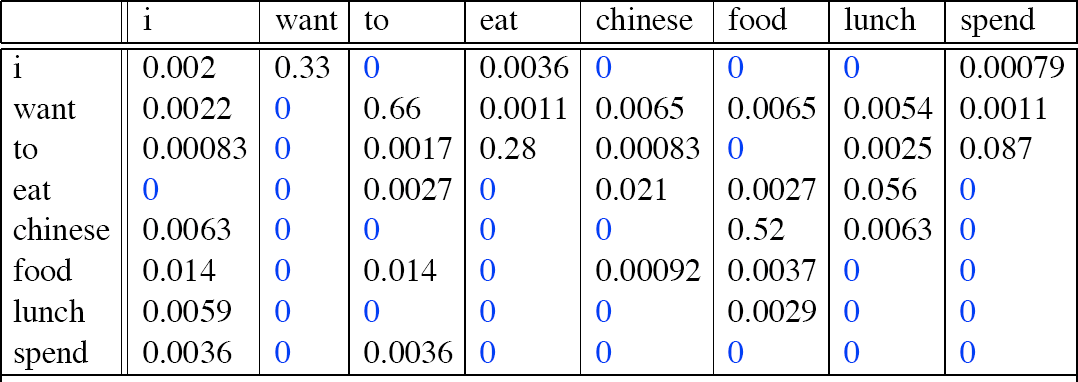
\includegraphics[width=0.85\textwidth]{../figures/diagrams/m1_perplexity.png}
    \caption{Evaluating Language Models: Visual summary of perplexity concepts from Module 1 source material (Evaluating Language Models PPT).}
    \label{fig:m1_perplexity}
\end{figure}

\subsection{Smoothing, Interpolation, and Backoff}

A critical problem with Maximum Likelihood Estimation is that any n-gram that never appears in the finite training corpus receives a probability of zero. This is problematic for two reasons: first, it means the model will assign zero probability to any test sentence containing an unseen n-gram, making perplexity undefined (division by zero). Second, even if the test sentence does contain a zero-probability n-gram, the model is essentially declaring that this sequence is impossible, which is almost certainly wrong---there are many perfectly grammatical word sequences that simply did not happen to appear in the training data.

\textbf{Smoothing} (also called \textbf{discounting}) is the standard solution. Smoothing algorithms ``shave off'' a small amount of probability mass from the n-grams that were seen in training and redistribute that mass to the unseen n-grams, giving them small but non-zero probabilities.

\subsubsection{The Zero-Probability Problem}

Any finite training corpus will miss some perfectly acceptable word sequences. These missing sequences are called \textbf{zeros}. For example, a training corpus might contain ``ruby'' and ``slippers'' individually but never the phrase ``ruby slippers.'' If we encounter ``ruby slippers'' in the test data, a bigram model without smoothing would compute:
\[
P(\text{slippers} \mid \text{ruby}) = \frac{C(\text{ruby}, \text{slippers})}{C(\text{ruby})} = \frac{0}{C(\text{ruby})} = 0
\]

If any word in a sentence has zero probability, the entire sentence probability becomes zero, and we cannot compute perplexity at all because we would need to divide by zero.

\subsubsection{Laplace (Add-One) Smoothing}

The simplest smoothing method is \textbf{Laplace smoothing}, also called \textbf{add-one smoothing}. The idea is to add one to the count of every n-gram before normalizing. Every n-gram that previously had a count of zero now has a count of one; every n-gram that previously had count $k$ now has count $k+1$.

For unigrams:
\[
P_{\text{Laplace}}(w_i) = \frac{c_i + 1}{N + V}
\]
where $c_i$ is the count of word $w_i$, $N$ is the total number of word tokens, and $V$ is the vocabulary size. The denominator increases by $V$ because we added one to the count of each of the $V$ vocabulary words.

For bigrams:
\[
P_{\text{Laplace}}(w_n \mid w_{n-1}) = \frac{C(w_{n-1}, w_n) + 1}{C(w_{n-1}) + V}
\]

Laplace smoothing is easy to understand and implement, but it tends to move too much probability mass to unseen events, making it impractical for modern language modeling. It remains useful, however, as a baseline and for text classification tasks where the smoothing behavior is less critical.

\begin{tcolorbox}[colback=green!5!white,colframe=green!75!black,title=\textbf{Numerical: Laplace Smoothing Example}]
\textbf{Given}: Berkeley Restaurant Project corpus with $V = 1446$.

Original bigram count for ``want to'': $C(\text{want}, \text{to}) = 608$, $C(\text{want}) = 927$.
\[
P_{\text{MLE}}(\text{to} \mid \text{want}) = \frac{608}{927} = 0.66
\]

After Laplace smoothing:
\[
P_{\text{Laplace}}(\text{to} \mid \text{want}) = \frac{608 + 1}{927 + 1446} = \frac{609}{2373} = 0.26
\]

\textbf{Observation}: Laplace smoothing reduces the probability of frequent bigrams dramatically (from 0.66 to 0.26) while giving unseen bigrams a small probability of $\frac{1}{2373} \approx 0.00042$. This is generally too aggressive for language modeling.
\end{tcolorbox}

\subsubsection{Add-k Smoothing}

An alternative to add-one smoothing is to add a smaller fractional count $k$ (where $0 < k < 1$), typically values like $0.5$ or $0.01$. This method is called \textbf{add-k smoothing}:
\[
P_{\text{Add-k}}(w_n \mid w_{n-1}) = \frac{C(w_{n-1}, w_n) + k}{C(w_{n-1}) + kV}
\]

The optimal value of $k$ depends on the corpus and task and can be determined by optimizing on a development set. While add-k smoothing is an improvement over Laplace smoothing, it still does not perform well for language modeling in practice because it produces counts with poor variance and inappropriate discounts for different frequency ranges.

\subsubsection{Language Model Interpolation}

\textbf{Interpolation} is a more sophisticated approach that combines probabilities from n-gram models of different orders. The intuition is that if a particular trigram has never been seen, we might still have useful information from the corresponding bigram or unigram. For example, even if we have never seen the trigram ``natural language processing'', we might have seen ``language processing'' as a bigram, which gives us some useful predictive power.

In simple linear interpolation, we combine unigram, bigram, and trigram probabilities with weights $\lambda_1, \lambda_2, \lambda_3$:
\[
\hat{P}(w_n \mid w_{n-2}, w_{n-1}) = \lambda_1 P(w_n) + \lambda_2 P(w_n \mid w_{n-1}) + \lambda_3 P(w_n \mid w_{n-2}, w_{n-1})
\]
where $\lambda_1 + \lambda_2 + \lambda_3 = 1$. The $\lambda$ values are typically learned from a held-out corpus by choosing the values that maximize the likelihood of that held-out data.

\subsubsection{Stupid Backoff}

\textbf{Backoff} is another alternative to interpolation. In a backoff model, if the n-gram we need has zero counts, we ``back off'' to a lower-order n-gram. \textbf{Stupid backoff} is a particularly simple version that does not attempt to normalize the backed-off probabilities into a true probability distribution. It simply uses a fixed weight $\lambda$ (typically 0.4) to scale the lower-order probability:
\[
S(w_i \mid w_{i-N+1:i-1}) =
\begin{cases}
\frac{\text{count}(w_{i-N+1:i})}{\text{count}(w_{i-N+1:i-1})} & \text{if count} > 0 \\
\lambda \cdot S(w_i \mid w_{i-N+2:i-1}) & \text{otherwise}
\end{cases}
\]

Stupid backoff is widely used in large-scale language modeling because it is simple, fast, and performs well in practice despite not being a proper probability distribution.

\subsection{Entropy and Cross-Entropy}

The perplexity measure actually arises from the information-theoretic concept of \textbf{cross-entropy}, which provides a deeper theoretical foundation for understanding why perplexity has the form it does.

\textbf{Entropy} $H(X)$ of a random variable $X$ measures the average amount of information (in bits) needed to encode outcomes of $X$:
\[
H(X) = -\sum_{x \in \chi} p(x) \log_2 p(x)
\]

For a sequence of words, we can define the \textbf{entropy rate} as the per-word entropy:
\[
H(L) = \lim_{n \to \infty} -\frac{1}{n} \log_2 P(w_1, w_2, \ldots, w_n)
\]

\textbf{Cross-entropy} $H(p, m)$ measures the average number of bits needed to encode outcomes from distribution $p$ using a model $m$:
\[
H(p, m) = \lim_{n \to \infty} -\frac{1}{n} \log_2 m(w_1, w_2, \ldots, w_n)
\]

The key insight is that perplexity is simply 2 raised to the power of cross-entropy:
\[
\text{Perplexity}(W) = 2^{H(W)}
\]

This explains why perplexity uses the inverse probability and why lower perplexity corresponds to a better model.

\begin{tcolorbox}[colback=green!5!white,colframe=green!75!black,title=\textbf{Numerical: Entropy of a Horse Race}]
\textbf{Given}: 8 horses with the following probabilities:
\begin{center}
\begin{tabular}{|c|c|c|c|c|c|c|c|}
\hline
Horse1 & Horse2 & Horse3 & Horse4 & Horse5 & Horse6 & Horse7 & Horse8 \\ \hline
$\frac{1}{2}$ & $\frac{1}{4}$ & $\frac{1}{8}$ & $\frac{1}{16}$ & $\frac{1}{64}$ & $\frac{1}{64}$ & $\frac{1}{64}$ & $\frac{1}{64}$ \\ \hline
\end{tabular}
\end{center}

\[
H(X) = -\frac{1}{2}\log_2\frac{1}{2} - \frac{1}{4}\log_2\frac{1}{4} - \frac{1}{8}\log_2\frac{1}{8} - \frac{1}{16}\log_2\frac{1}{16} - 4 \times \frac{1}{64}\log_2\frac{1}{64}
\]
\[
H(X) = 0.5 + 0.5 + 0.375 + 0.25 + 4 \times 0.09375 = 2 \text{ bits}
\]

For 8 equally likely horses, the entropy would be $\log_2 8 = 3$ bits. The non-uniform distribution requires fewer bits to encode because some outcomes are highly predictable.
\end{tcolorbox}

\subsection{Edit Distance}

\textbf{Edit distance} (also known as Levenshtein distance) measures the minimum number of single-character editing operations required to transform one string into another. The three allowed operations are:
\begin{itemize}
    \item \textbf{Insertion}: Insert a character into the string.
    \item \textbf{Deletion}: Delete a character from the string.
    \item \textbf{Substitution}: Replace one character with another.
\end{itemize}

Edit distance is computed efficiently using \textbf{dynamic programming}. We construct a matrix $D$ where $D[i, j]$ represents the edit distance between the first $i$ characters of the source string and the first $j$ characters of the target string. The recurrence relation is:
\[
D[i, j] = \min\begin{cases}
D[i-1, j] + 1 & \text{(deletion)} \\
D[i, j-1] + 1 & \text{(insertion)} \\
D[i-1, j-1] + \text{cost}(i,j) & \text{(substitution)}
\end{cases}
\]
where $\text{cost}(i,j) = 0$ if the $i$-th source character equals the $j$-th target character, and $1$ (or $2$) otherwise. The base cases are $D[0, j] = j$ and $D[i, 0] = i$.

\begin{tcolorbox}[colback=green!5!white,colframe=green!75!black,title=\textbf{Numerical: Edit Distance Example}]
\textbf{Given}: Source = ``intention'', Target = ``execution''

The minimum edit distance is 5 operations (with substitution cost = 2):
\begin{enumerate}
    \item \textbf{Delete} ``i'': intention $\to$ ntention
    \item \textbf{Substitute} ``n'' $\to$ ``e'': ntention $\to$ etention
    \item \textbf{Substitute} ``t'' $\to$ ``x'': etention $\to$ exention
    \item \textbf{Insert} ``u'': exention $\to$ exenution
    \item \textbf{Substitute} ``n'' $\to$ ``c'': exenution $\to$ execution
\end{enumerate}
\textbf{Total cost}: 1 (delete) + 2 (sub) + 2 (sub) + 1 (insert) + 2 (sub) = 8 (with cost=1 for substitution) or 5 (with cost=2 for substitution and counting operations).
\end{tcolorbox}

\begin{figure}[H]
    \centering
    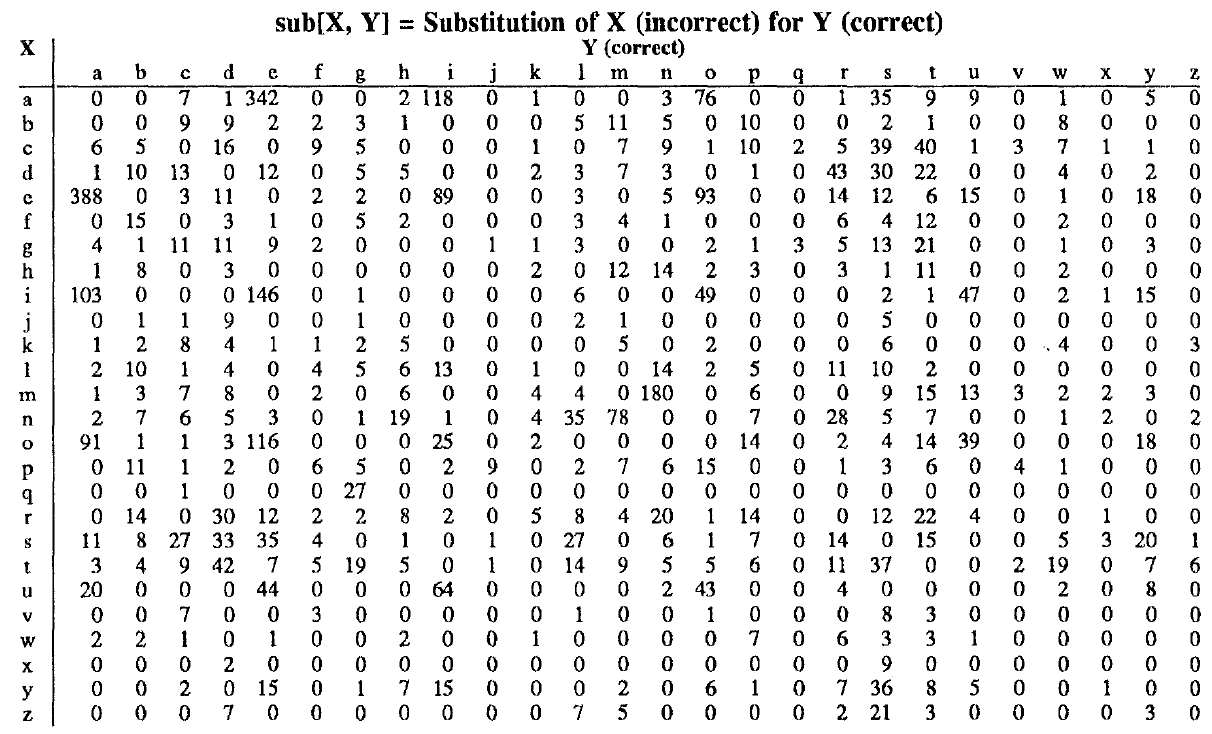
\includegraphics[width=0.85\textwidth]{../figures/diagrams/m1_edit_distance.png}
    \caption{Edit Distance visualization from source material (EditDistance.pptx), showing the dynamic programming matrix and alignment path between two strings.}
    \label{fig:m1_edit_distance}
\end{figure}


\newpage

\section{Module 2: Word Senses, WordNet, and Vector Semantics}

\subsection{Word Senses and Polysemy}

When we encounter a word in natural language, we rarely think about the fact that most words carry multiple meanings. The study of how words relate to meaning begins with understanding that a \textbf{word sense} is a discrete representation of one aspect of the meaning of a word. For example, the word ``bank'' can refer to a financial institution (``I deposited money at the bank'') or the edge of a river (``We sat on the bank of the river''). Each of these is a distinct sense of the word ``bank.''

The phenomenon of a single word having multiple related meanings is called \textbf{polysemy}. Polysemy is different from \textbf{homonymy}, where two words happen to share the same spelling and pronunciation but have completely unrelated meanings (e.g., ``bark'' as the sound a dog makes vs. ``bark'' as the outer covering of a tree). In polysemy, the different senses of a word are usually related in some way. For instance, the financial ``bank'' and the river ``bank'' both relate to the concept of an edge or boundary---financial institutions were historically located on the edges of marketplaces.

\textbf{Structured polysemy} refers to the systematic relationships that exist between the senses of a polysemous word. For example, the word ``newspaper'' can refer to the physical object (``The newspaper fell off the table'') or the organization that produces it (``The newspaper published an editorial''). The relationship between these two senses is a regular metonymic pattern (ORGANIZATION $\leftrightarrow$ PHYSICAL ARTIFACT) that applies to many words.

Word senses can be distinguished by several criteria:
\begin{itemize}
    \item \textbf{Independent truth conditions}: Two senses are distinct if a sentence can be simultaneously true under one sense and false under another. For example, ``The newspaper is on the table'' is true if ``newspaper'' means the physical object, but false if it means the organization.
    \item \textbf{Different syntactic behavior}: Distinct senses may have different grammatical properties. For example, ``book'' as a noun takes plural form (``books''), while ``book'' as a verb takes past tense (``booked'').
    \item \textbf{Independent sense relations}: Each sense may participate in different lexical relations. For example, ``bank'' (financial institution) is a hyponym of ``financial institution'', while ``bank'' (river edge) is a hyponym of ``shore''.
    \item \textbf{Antagonistic meanings (zeugma test)}: If a sentence uses a word in two incompatible senses simultaneously, the result is anomalous. For example, ``?He withdrew the money from the bank and sat on it'' is zeugmatic because ``bank'' is being used as both a financial institution and a river edge.
\end{itemize}

\subsection{Relations Between Senses}

Lexical semantics is concerned with the relationships that hold between the meanings of words. Understanding these relationships is essential for tasks ranging from information retrieval to machine translation to question answering.

\subsubsection{Synonymy}

Two word senses are \textbf{synonyms} if they are identical or nearly identical in meaning, such that they can be substituted for each other in many (though not necessarily all) contexts without changing the truth conditions of the sentence. Examples include ``couch'' and ``sofa'', ``vomit'' and ``throw up'', and ``car'' and ``automobile''.

It is important to note that synonymy is a relationship between \textit{senses}, not between words. Two words may be synonyms in some senses but not in others. For example, ``big'' and ``large'' are synonyms when describing physical size, but only ``large'' can describe the scope of an investigation (``a large investigation'' sounds natural, while ``?a big investigation'' is slightly less formal).

True absolute synonymy is rare because words that are very close in meaning usually differ in register (formal vs. informal), dialect, or connotation. Near-synonyms like ``ask'' and ``request'' or ``error'' and ``mistake'' illustrate this subtlety.

\subsubsection{Antonymy}

\textbf{Antonyms} are words with opposite meanings. Unlike synonymy, antonymy is a relationship between words rather than senses, because a word typically has only one antonym for each sense. Common examples include ``long''/``short'', ``big''/``little'', ``fast''/``slow'', ``cold''/``hot'', and ``rise''/``fall''.

A special class of antonyms called \textbf{reversives} describes changes or movements in opposite directions. Examples include ``rise''/``fall'', ``up''/``down'', and ``advance''/``retreat''. These are particularly important in temporal and spatial descriptions.

\subsubsection{Taxonomic Relations: Hyponymy and Hypernymy}

\textbf{Hyponymy} and \textbf{hypernymy} describe the relationship between a more specific concept and a more general concept. A \textbf{hyponym} is a word that denotes a subclass of another word. For example, ``car'' is a hyponym of ``vehicle'' because every car is a vehicle. A \textbf{hypernym} (also called a \textbf{superordinate}) is the more general word; ``vehicle'' is a hypernym of ``car''.

The relationship is often expressed as an \textbf{IS-A hierarchy}: ``A car IS-A vehicle.'' This hierarchical structure is fundamental to organizing lexical knowledge because it allows inference: if we know something is a car, we automatically know it is also a vehicle and inherits all the properties of vehicles.

\subsubsection{Meronymy}

\textbf{Meronymy} is the part-whole relationship. A \textbf{meronym} is a part of something. For example, a ``wheel'' is a meronym of ``car'', and a ``leg'' is a meronym of ``chair''. Conversely, the whole is called a \textbf{holonym}: ``car'' is a holonym of ``wheel''. Meronymy is important for understanding physical descriptions and for tasks like question answering (e.g., ``How many wheels does a car have?'' requires knowing the meronymy relationship).

\subsection{WordNet}

\textbf{WordNet} is a large, freely available lexical database of English (and other languages) that organizes words into synonym sets called \textbf{synsets}. Rather than listing words alphabetically like a traditional dictionary, WordNet groups words into synsets based on their meanings and defines relationships between these synsets.

The English WordNet consists of three separate databases:
\begin{itemize}
    \item \textbf{Nouns}: 117,798 entries in WordNet 3.0
    \item \textbf{Verbs}: 11,529 entries
    \item \textbf{Adjectives and adverbs}: 22,479 adjectives and 4,481 adverbs
\end{itemize}

Each synset in WordNet represents a single underlying lexical concept and is associated with a \textbf{gloss} (a short textual definition) and often example sentences. For example, the synset for the noun sense of ``bank'' meaning a financial institution might have the gloss: ``a financial institution that accepts deposits and channels the money into lending activities.''

WordNet also organizes concepts into \textbf{supersenses}, which are lexicographic categories that provide a coarse-grained semantic classification. There are 26 supersenses for nouns (e.g., ANIMAL, ARTIFACT, FOOD, PERSON) and 15 for verbs (e.g., COMMUNICATION, COMPETITION, CONSUMPTION).

\subsubsection{Sense Relations in WordNet}

WordNet encodes many of the lexical relations discussed above at the sense level. The following table summarizes the major relations:
\begin{center}
\begin{tabular}{|l|l|l|}
\hline
\textbf{Relation} & \textbf{Also Called} & \textbf{Example} \\ \hline
Hypernym & Superordinate & breakfast$^1$ $\to$ meal$^1$ \\ \hline
Hyponym & Subordinate & meal$^1$ $\to$ lunch$^1$ \\ \hline
Instance Hypernym & Instance & Austen$^1$ $\to$ author$^1$ \\ \hline
Part Meronym & Has-Part & table$^2$ $\to$ leg$^3$ \\ \hline
Antonym & Semantic opposition & leader$^1$ $\Leftrightarrow$ follower$^1$ \\ \hline
Derivation & Same morphological root & destruction$^1$ $\Leftrightarrow$ destroy$^1$ \\ \hline
\end{tabular}
\end{center}

\begin{figure}[H]
    \centering
    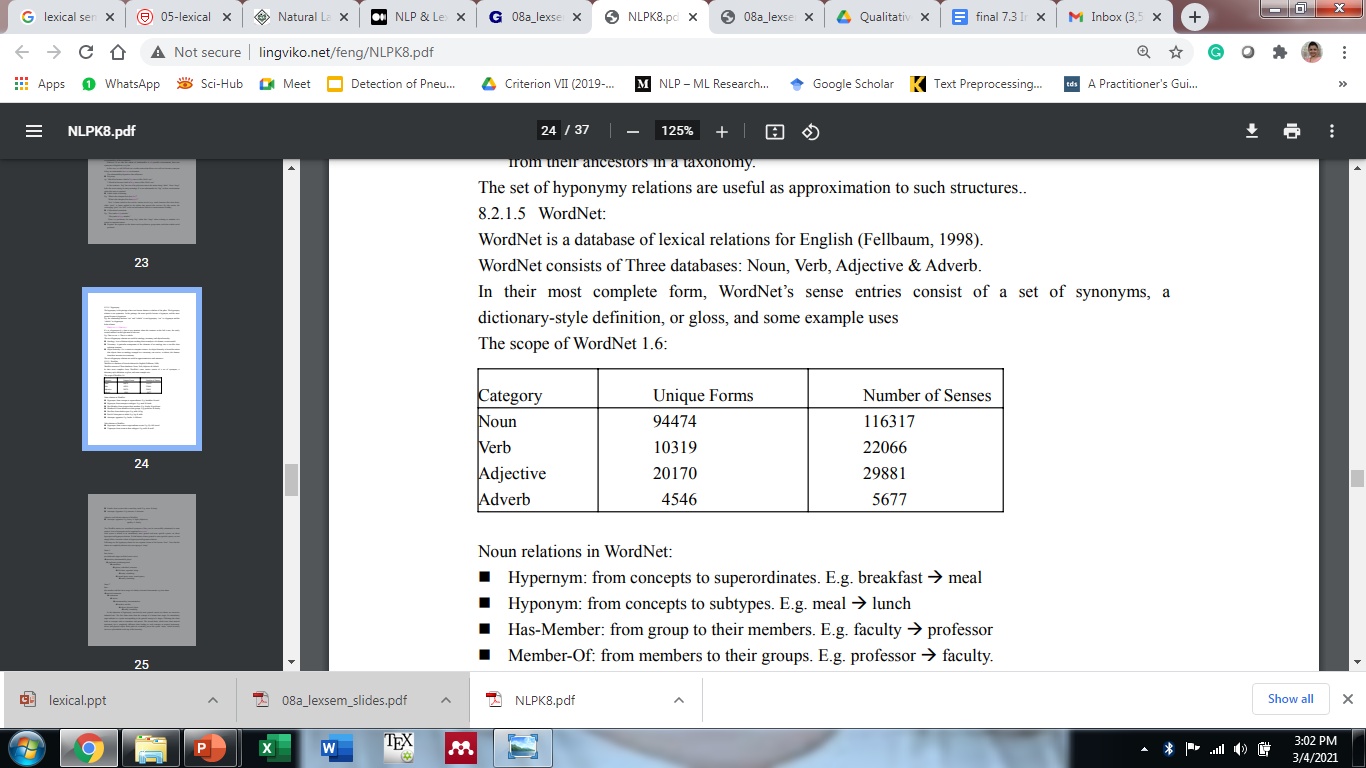
\includegraphics[width=0.85\textwidth]{../figures/diagrams/m2_word_sense.png}
    \caption{Word Sense and Semantic Relations visualization from source material (Word Sense Disambiguation PPT), showing the structure of sense relations and disambiguation concepts.}
    \label{fig:m2_word_sense}
\end{figure}

\subsection{Word Sense Disambiguation (WSD)}

\textbf{Word Sense Disambiguation (WSD)} is the computational task of determining which sense of a word is being used in a particular context. Because most common words are polysemous, WSD is essential for many NLP applications that require understanding the precise meaning of text.

WSD tasks come in two main varieties:
\begin{itemize}
    \item \textbf{Lexical sample task}: A small, pre-selected set of target words is chosen, and the system must disambiguate only those words. Because the inventory of senses is small, this task is more tractable and simple supervised classification approaches work well.
    \item \textbf{All-words task}: The system must disambiguate every content word in a text. This is much harder because the set of possible senses is much larger, leading to data sparsity problems.
\end{itemize}

\subsubsection{WSD Algorithms}

Several approaches have been developed for WSD, ranging from simple baselines to sophisticated neural methods:

\begin{enumerate}
    \item \textbf{Most Frequent Sense Baseline}: This simple but surprisingly effective baseline always chooses the most frequent sense of a word from a labeled corpus. In WordNet, senses are ordered by frequency, so this corresponds to choosing the first sense. This baseline achieves roughly 60-70\% accuracy, which is difficult to beat for many words.
    \item \textbf{One Sense Per Discourse}: This heuristic, based on the observation that a word appearing multiple times in a text or discourse often appears with the same sense, provides a useful bias toward consistent sense assignment within a document.
    \item \textbf{Contextual Embeddings (State of the Art)}: The best-performing WSD algorithm is a simple 1-nearest-neighbor approach using contextual word embeddings such as BERT. At training time, each labeled sentence is passed through BERT to produce a contextual embedding for the target word. At test time, the contextual embedding of the target word is compared to all sense embeddings, and the nearest neighbor is chosen as the predicted sense.
    \item \textbf{Simplified Lesk Algorithm}: This knowledge-based approach chooses the sense whose dictionary gloss and example sentences share the most words with the target word's surrounding context. For example, to disambiguate ``bank'' in ``The bank can guarantee deposits will cover future tuition costs'', the algorithm compares the context words to the glosses of each sense and selects the one with the highest word overlap.
\end{enumerate}

\subsection{Pointwise Mutual Information (PMI)}

\textbf{Pointwise Mutual Information (PMI)} is a measure of association between two events (or in NLP, between two words) that quantifies how much more they co-occur than would be expected by chance if they were independent. PMI is a fundamental tool in distributional semantics, the branch of semantics that studies word meaning based on patterns of word co-occurrence in large corpora.

The intuition behind PMI is straightforward: if two words appear together much more often than their individual frequencies would predict, they are likely semantically related. For example, ``doctor'' and ``nurse'' co-occur far more often than chance, suggesting a strong semantic association.

The formula for PMI between a target word $w$ and a context word $c$ is:
\[
\text{PMI}(w, c) = \log_2 \frac{P(w, c)}{P(w)P(c)}
\]

where $P(w, c)$ is the probability that $w$ and $c$ co-occur, $P(w)$ is the probability of $w$, and $P(c)$ is the probability of $c$. When $w$ and $c$ are independent, $P(w, c) = P(w)P(c)$, and PMI equals zero. Positive PMI values indicate positive association (they co-occur more than expected); negative PMI values indicate negative association (they co-occur less than expected).

\textbf{Positive PMI (PPMI)} is a variant that replaces negative PMI values with zero, since negative associations are often noisy and not semantically meaningful in practice:
\[
\text{PPMI}(w, c) = \max\left(\log_2 \frac{P(w, c)}{P(w)P(c)}, 0\right)
\]

\begin{tcolorbox}[colback=green!5!white,colframe=green!75!black,title=\textbf{Numerical: PPMI Calculation}]
\textbf{Given}: Co-occurrence counts from a Wikipedia corpus:
\begin{center}
\begin{tabular}{|l|c|c|c|c|c|c|}
\hline
 & computer & data & result & pie & sugar & count(w) \\ \hline
cherry & 2 & 8 & 9 & 442 & 25 & 486 \\ \hline
strawberry & 0 & 0 & 1 & 60 & 19 & 80 \\ \hline
digital & 1670 & 1683 & 85 & 5 & 4 & 3447 \\ \hline
information & 3325 & 3982 & 378 & 5 & 13 & 7703 \\ \hline
count(c) & 4997 & 5673 & 473 & 512 & 61 & 11716 \\ \hline
\end{tabular}
\end{center}

\textbf{Calculate PPMI(information, data)}:

Joint probability:
\[
P(w=\text{information}, c=\text{data}) = \frac{3982}{11716} = 0.3399
\]

Marginal probabilities:
\[
P(w=\text{information}) = \frac{7703}{11716} = 0.6575, \quad
P(c=\text{data}) = \frac{5673}{11716} = 0.4842
\]

PMI:
\[
\text{PMI}(\text{information}, \text{data}) = \log_2 \frac{0.3399}{0.6575 \times 0.4842} = \log_2(1.067) = 0.0944
\]

Since PMI is positive, PPMI equals PMI: $\text{PPMI}(\text{information}, \text{data}) = 0.0944$.
\end{tcolorbox}

\begin{figure}[H]
    \centering
    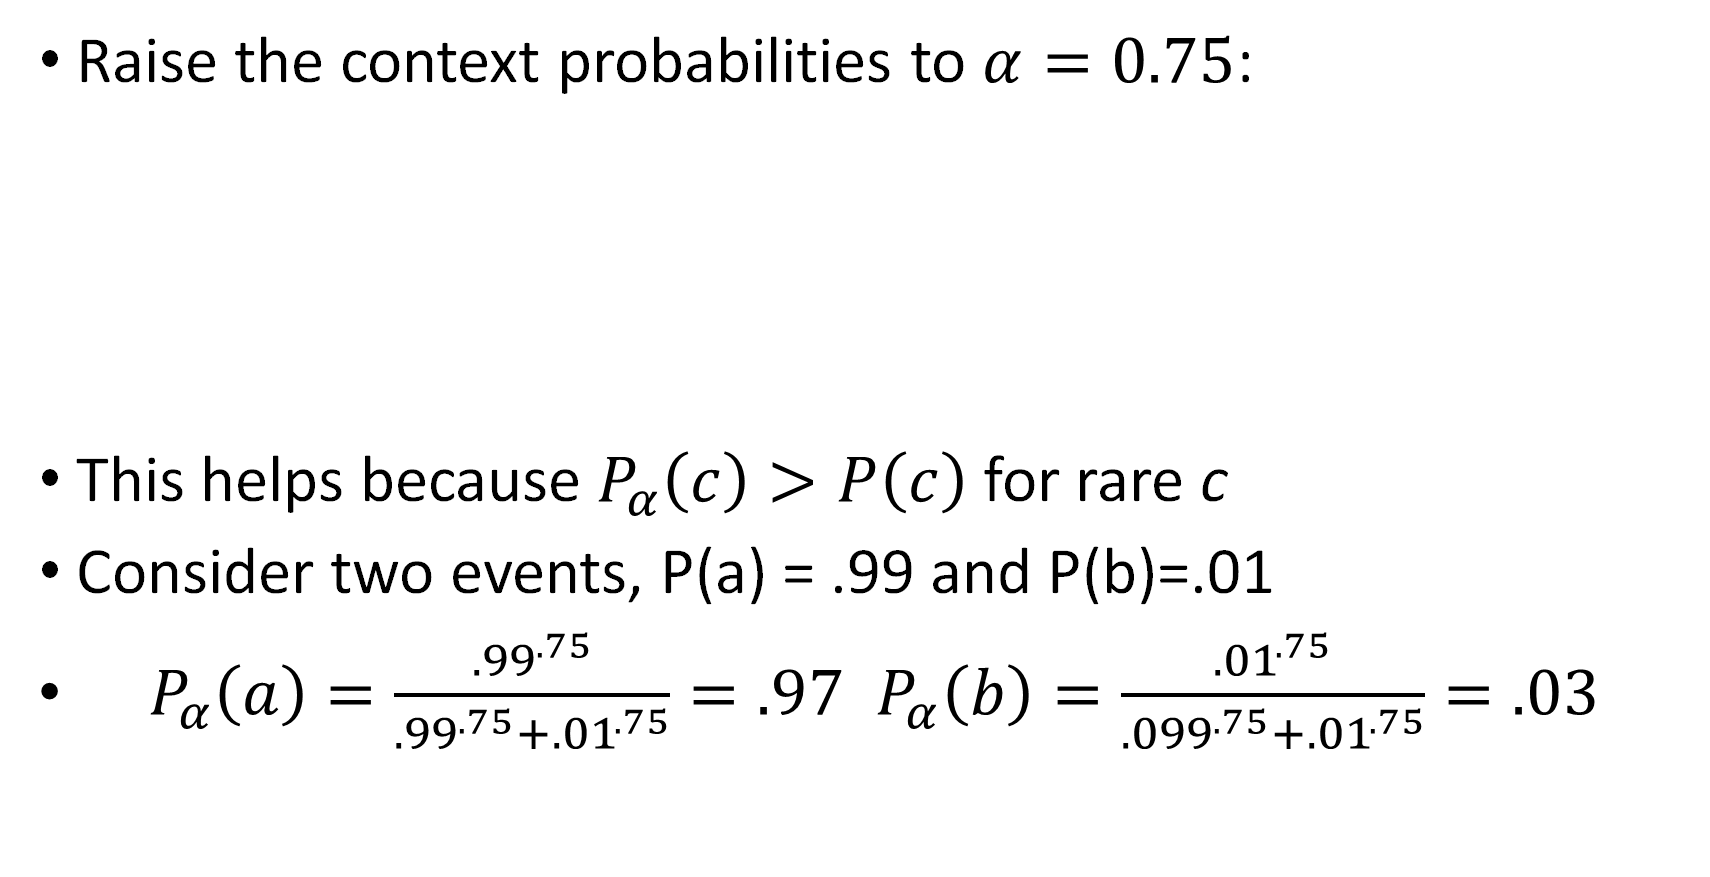
\includegraphics[width=0.85\textwidth]{../figures/diagrams/m2_vector_semantics.png}
    \caption{Vector Semantics and Distributional Hypothesis visualization from source material (Vector Semantics PPT), illustrating how word meaning is represented in vector spaces based on co-occurrence patterns.}
    \label{fig:m2_vector_semantics}
\end{figure}

\subsection{Word Sense Induction (WSI)}

\textbf{Word Sense Induction (WSI)} is the unsupervised counterpart to WSD. Instead of using a pre-defined inventory of senses (like WordNet), WSI algorithms automatically discover the senses of a word from corpus data. This is valuable because building sense-labeled corpora is expensive and time-consuming, and the optimal sense granularity may differ across applications.

Most WSI algorithms follow the early work of Sch\"utze (1992, 1998) and use clustering over word embeddings:
\begin{enumerate}
    \item \textbf{Training phase}: For each token of the target word in a corpus, compute a context vector representing the words that appear near the target word.
    \item \textbf{Clustering}: Apply a clustering algorithm (such as agglomerative clustering or k-means) to group these context vectors into a predefined number of clusters. Each cluster represents an automatically induced sense.
    \item \textbf{Sense representation}: Compute the centroid (average vector) of each cluster. This centroid becomes the sense vector representing that induced sense.
\end{enumerate}

At test time, to disambiguate a new occurrence of the target word, we compute its context vector and assign it to the cluster whose centroid is closest, using cosine similarity or Euclidean distance as the distance metric.

\begin{figure}[H]
    \centering
    
\includegraphics[width=0.85\textwidth]{../figures/diagrams/m2_semantic_analysis.png}
    \caption{Semantic Analysis framework visualization from source material (SemanticAnalysisPart2 PPT), showing the pipeline from raw text to semantic representations.}
    \label{fig:m2_semantic_analysis}
\end{figure}


\newpage

\section{Module 3: Naive Bayes and Text Classification}

\subsection{Introduction to Text Classification}

\textbf{Text classification} (also called text categorization) is the task of assigning a predefined label or category to an entire text or document based on its content. This is one of the most fundamental and widely applied tasks in natural language processing, forming the backbone of systems that must automatically organize, filter, or analyze large volumes of text.

The applications of text classification are extensive and touch nearly every domain where text is processed at scale:
\begin{itemize}
    \item \textbf{Sentiment Analysis}: Determining whether a piece of text (such as a product review, tweet, or movie review) expresses a positive, negative, or neutral sentiment. This is crucial for businesses monitoring customer feedback, for political analysts tracking public opinion, and for financial traders gauging market sentiment.
    \item \textbf{Spam Detection}: Classifying incoming emails as spam or legitimate (ham). This is one of the oldest and most successful applications of text classification, saving billions of hours of human attention.
    \item \textbf{Language Identification}: Automatically determining which language a given piece of text is written in. This is essential for multilingual search engines, translation services, and content filtering systems.
    \item \textbf{Authorship Attribution}: Determining the author of a text based on stylistic features. This has applications in forensic linguistics, plagiarism detection, and literary analysis.
    \item \textbf{Subject Categorization}: Assigning library subject categories, news article topics, or patent classifications to documents. This enables efficient information retrieval and knowledge organization.
\end{itemize}

Text classification is typically formulated as a supervised learning problem: given a training set of documents labeled with their correct categories, we learn a function that maps new, unlabeled documents to categories.

\subsection{Naive Bayes Classifiers}

The \textbf{Naive Bayes classifier} is one of the simplest yet most effective text classification algorithms. Despite its simplifying assumptions, it often performs surprisingly well on text data and serves as a strong baseline against which more complex models are compared.

Naive Bayes is a \textbf{generative classifier}. Unlike discriminative classifiers (such as logistic regression or SVMs), which directly model the decision boundary between classes, generative classifiers build a model of how each class could have generated the observed data. The name ``Naive Bayes'' comes from two sources: ``Bayes'' because the classifier is derived from Bayes' theorem, and ``Naive'' because it makes a strong simplifying assumption about the independence of features.

\subsubsection{Bayes' Rule and the Classification Decision}

At the heart of the Naive Bayes classifier is \textbf{Bayes' rule} (also called Bayes' theorem), which relates the conditional and marginal probabilities of random events:
\[
P(c \mid d) = \frac{P(d \mid c) P(c)}{P(d)}
\]

In the context of text classification:
\begin{itemize}
    \item $c$ represents a class (e.g., ``positive'' or ``negative'' for sentiment analysis)
    \item $d$ represents a document
    \item $P(c)$ is the \textbf{prior probability} of class $c$ (how likely the class is before seeing the document)
    \item $P(d \mid c)$ is the \textbf{likelihood} (how likely the document is if the class is $c$)
    \item $P(c \mid d)$ is the \textbf{posterior probability} (how likely the class is after seeing the document)
\end{itemize}

Because $P(d)$ is the same for all classes, it does not affect which class is most probable. Therefore, the classifier simply returns the class with the maximum posterior:
\[
\hat{c} = \arg\max_{c \in C} P(c \mid d) = \arg\max_{c \in C} P(d \mid c) P(c)
\]

\subsubsection{The Bag of Words Assumption}

To make the computation of $P(d \mid c)$ tractable, the Naive Bayes classifier makes the \textbf{bag of words assumption}: a document is represented as an unordered set (or multiset) of words with their frequencies. The position of words in the document is completely ignored---only the identity and frequency of words matter.

For example, under the bag of words assumption, the sentences ``The movie was good, not bad at all'' and ``The movie was bad, not good at all'' would have identical representations, even though their meanings are opposite. This is clearly a severe simplification, but it works surprisingly well in practice for many classification tasks because the overall word frequencies often carry enough signal to distinguish classes.

\subsubsection{The Naive Bayes Assumption: Conditional Independence}

The second and more critical assumption is the \textbf{conditional independence assumption}: given the class label, the probability of each word occurring in the document is independent of the probabilities of all other words. Formally:
\[
P(f_1, f_2, \ldots, f_n \mid c) = P(f_1 \mid c) \times P(f_2 \mid c) \times \cdots \times P(f_n \mid c)
\]

This assumption is ``naive'' because in natural language, words are clearly not independent---``New'' and ``York'' co-occur far more often than chance would predict, and ``not'' strongly influences the interpretation of nearby words. However, the conditional independence assumption dramatically reduces the number of parameters that must be estimated from data and often leads to robust classifiers that generalize well.

Combining the bag of words and conditional independence assumptions, the Naive Bayes classification rule becomes:
\[
c_{NB} = \arg\max_{c \in C} P(c) \prod_{f \in F} P(f \mid c)
\]

where $F$ is the set of feature values (word occurrences) in the document, and $f$ ranges over the words (or word features) in the document.

\subsubsection{Training the Naive Bayes Classifier}

Training a Naive Bayes classifier involves estimating the probabilities $P(c)$ and $P(f \mid c)$ from the training data using Maximum Likelihood Estimation with Laplace smoothing.

The \textbf{class prior} $P(c)$ is estimated as the proportion of training documents that belong to class $c$:
\[
\hat{P}(c) = \frac{N_c}{N_{doc}}
\]
where $N_c$ is the number of training documents in class $c$ and $N_{doc}$ is the total number of training documents.

The \textbf{likelihood} $\hat{P}(w_i \mid c)$ is estimated from the word counts in the training documents of class $c$. To handle words that never appeared in the training documents of a particular class (which would cause the entire product to become zero), we use \textbf{add-one (Laplace) smoothing}:
\[
\hat{P}(w_i \mid c) = \frac{\text{count}(w_i, c) + 1}{\sum_{w \in V} (\text{count}(w, c) + 1)} = \frac{\text{count}(w_i, c) + 1}{\sum_{w \in V} \text{count}(w, c) + |V|}
\]

where $|V|$ is the vocabulary size. The $+1$ in the numerator ensures that every word has a non-zero probability, and the $+|V|$ in the denominator ensures that the probabilities sum to 1.

\begin{tcolorbox}[colback=green!5!white,colframe=green!75!black,title=\textbf{Numerical: Naive Bayes Sentiment Classification}]
\textbf{Training Data}:
\begin{center}
\begin{tabular}{|c|l|}
\hline
\textbf{Class} & \textbf{Document} \\ \hline
- & just plain boring \\ \hline
- & entirely predictable and lacks energy \\ \hline
- & no surprises and very few laughs \\ \hline
+ & very powerful \\ \hline
+ & the most fun film of the summer \\ \hline
\end{tabular}
\end{center}

\textbf{Test sentence}: ``predictable with no fun''

\textbf{Step 1}: Compute prior probabilities
\[
P(-) = \frac{3}{5} = 0.6, \quad P(+) = \frac{2}{5} = 0.4
\]

\textbf{Step 2}: Build vocabulary and compute word counts

Vocabulary (20 words): just, plain, boring, entirely, predictable, and, lacks, energy, no, surprises, very, few, laughs, powerful, the, most, fun, film, of, summer

Negative class total word count: 14 (just, plain, boring, entirely, predictable, and\texttimes2, lacks, energy, no, surprises, very, few, laughs)

Positive class total word count: 9 (very\texttimes2, powerful, the, most, fun, film, of, summer)

\textbf{Step 3}: Compute likelihoods with add-1 smoothing ($|V| = 20$)

For ``predictable'':
\[
P(\text{predictable} \mid -) = \frac{1+1}{14+20} = \frac{2}{34}, \quad
P(\text{predictable} \mid +) = \frac{0+1}{9+20} = \frac{1}{29}
\]

For ``no'':
\[
P(\text{no} \mid -) = \frac{1+1}{14+20} = \frac{2}{34}, \quad
P(\text{no} \mid +) = \frac{0+1}{9+20} = \frac{1}{29}
\]

For ``fun'':
\[
P(\text{fun} \mid -) = \frac{0+1}{14+20} = \frac{1}{34}, \quad
P(\text{fun} \mid +) = \frac{1+1}{9+20} = \frac{2}{29}
\]

\textbf{Step 4}: Compute posterior (ignoring ``with'' as unknown)
\[
P(-) \cdot P(S \mid -) = \frac{3}{5} \times \frac{2}{34} \times \frac{2}{34} \times \frac{1}{34} = \frac{12}{5 \times 39304} \approx 6.1 \times 10^{-5}
\]
\[
P(+) \cdot P(S \mid +) = \frac{2}{5} \times \frac{1}{29} \times \frac{1}{29} \times \frac{2}{29} = \frac{4}{5 \times 24389} \approx 3.2 \times 10^{-5}
\]

\textbf{Result}: Since $6.1 \times 10^{-5} > 3.2 \times 10^{-5}$, the negative class has higher posterior probability.\\
\textbf{Prediction}: \textbf{NEGATIVE sentiment}
\end{tcolorbox}

\subsection{Optimizations for Sentiment Analysis}

While the basic multinomial Naive Bayes classifier performs well, several optimizations have been developed specifically for sentiment analysis and other text classification tasks.

\subsubsection{Binary Multinomial Naive Bayes}

In standard multinomial Naive Bayes, word frequencies are counted---if a word appears 5 times in a document, it contributes 5 factors to the product. However, for sentiment analysis, \textbf{presence} often matters more than \textbf{frequency}. A review that mentions ``bad'' once and ``terrible'' once is more negative than one that mentions ``bad'' five times but no other negative words.

\textbf{Binary multinomial Naive Bayes} addresses this by clipping all word counts at 1. Each word is treated as either present or absent in the document, regardless of how many times it appears. This simple modification often improves classification accuracy for sentiment analysis because it reduces the influence of repeated words and focuses the model on the vocabulary of the document.

\subsubsection{Negation Handling}

One of the most important challenges in sentiment analysis is handling \textbf{negation}. Words like ``not'' and ``no'' can completely flip the sentiment of nearby words. For example, ``not good'' should be classified as negative, even though ``good'' is a positive word.

A simple but effective heuristic for handling negation is to prepend a ``NOT_'' prefix to every word that appears between a negation word (n't, not, no, never) and the next punctuation mark. For example, the sentence ``I did not like this movie'' becomes ``I did not NOT\_like NOT\_this NOT\_movie''. This creates new pseudo-words (``NOT\_like'', ``NOT\_this'') that the classifier can learn to associate with negative sentiment.

\subsubsection{Sentiment Lexicons}

\textbf{Sentiment lexicons} are pre-compiled dictionaries of words annotated with their sentiment polarity (positive, negative, or neutral). Incorporating lexicon features into a Naive Bayes classifier can improve performance, especially when training data is limited. Well-known sentiment lexicons include:
\begin{itemize}
    \item \textbf{General Inquirer}: A general-purpose lexicon with positive/negative annotations for thousands of English words.
    \item \textbf{LIWC (Linguistic Inquiry and Word Count)}: A commercial lexicon categorizing words into psychological and linguistic categories.
    \item \textbf{MPQA Subjectivity Lexicon}: A freely available lexicon of subjective words annotated with polarity.
\end{itemize}

\begin{figure}[H]
    \centering
    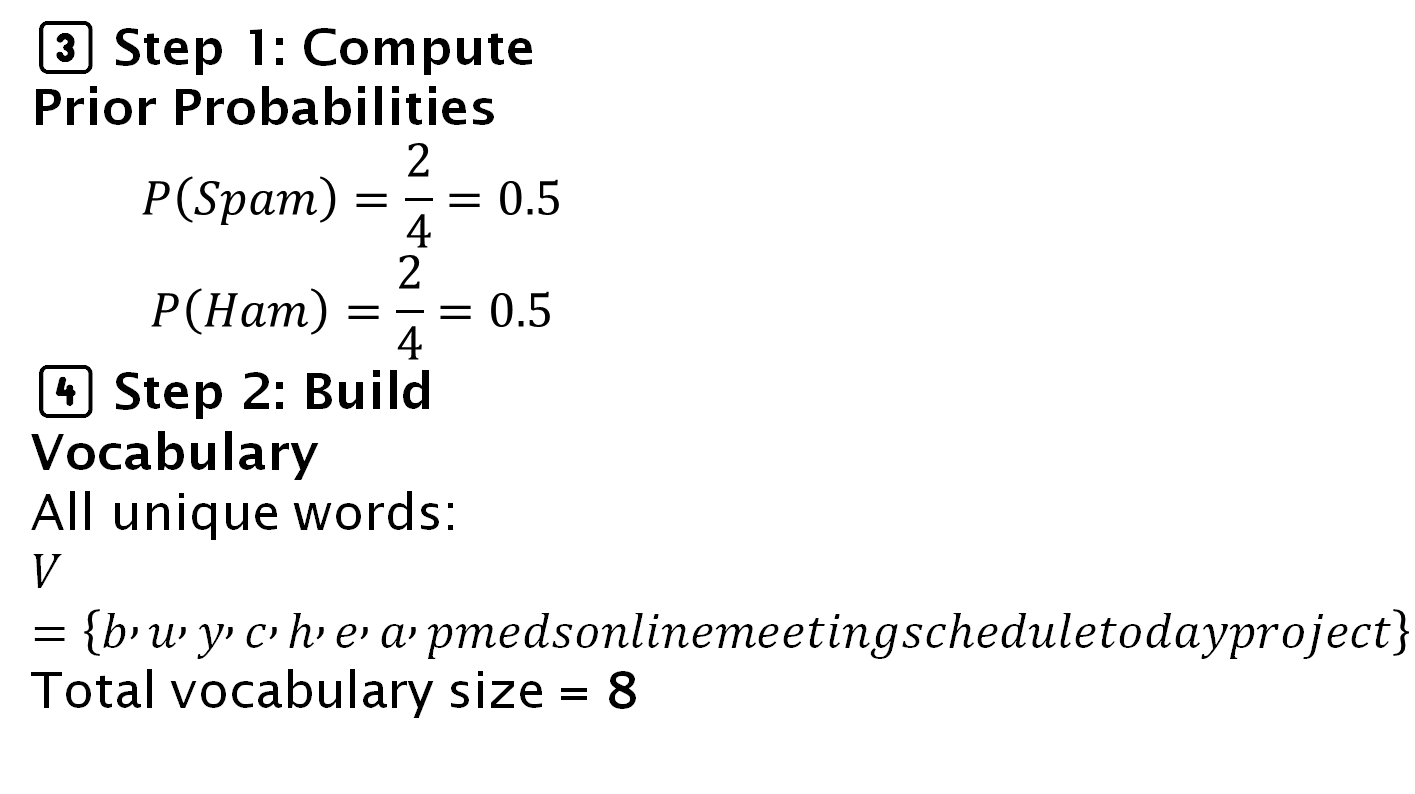
\includegraphics[width=0.85\textwidth]{../figures/diagrams/m3_naive_bayes.png}
    \caption{Naive Bayes Classifier architecture and text classification pipeline from source material (Text Classification using Naive Bayes PPT), illustrating the bag-of-words representation and probability estimation process.}
    \label{fig:m3_naive_bayes}
\end{figure}


\newpage

\section{Module 4: Deep Learning Architectures for Sequence Processing}

\subsection{Recurrent Neural Networks (RNNs)}

\textbf{Recurrent Neural Networks (RNNs)} are a class of artificial neural networks specifically designed to process sequential data. Unlike feedforward neural networks, which assume that all inputs are independent of each other, RNNs maintain an internal memory state that captures information about previous inputs in the sequence. This makes them uniquely suited for tasks involving natural language, speech, time series, and any other domain where the order of data matters.

The fundamental challenge that RNNs address is that standard feedforward networks require fixed-size inputs. A sentence of length 5 and a sentence of length 50 cannot both be fed into the same fixed-input network without some form of truncation, padding, or windowing. RNNs solve this by processing the sequence one element at a time, maintaining a hidden state that evolves as the network reads each new element. This allows RNNs to handle variable-length sequences naturally and to capture dependencies between elements at different positions in the sequence.

\subsubsection{RNN Architecture}

The architecture of a simple RNN consists of three sets of learnable weight matrices and a hidden state vector:
\begin{itemize}
    \item $W_x$: The \textbf{input-to-hidden} weight matrix, which transforms the input at the current time step into the hidden state space.
    \item $W_h$: The \textbf{hidden-to-hidden} (recurrent) weight matrix, which transforms the previous hidden state into the new hidden state. This is the key matrix that enables the network to maintain memory across time steps.
    \item $W_o$: The \textbf{hidden-to-output} weight matrix, which transforms the hidden state into the output space (e.g., a probability distribution over vocabulary words for language modeling).
\end{itemize}

At each time step $t$, the RNN receives an input vector $x_t$ (typically a word embedding) and updates its hidden state $h_t$ according to the following recurrence relation:
\[
h_t = \tanh(W_h h_{t-1} + W_x x_t + b_h)
\]

where $b_h$ is a bias vector and $\tanh$ is the hyperbolic tangent activation function, which squashes the values to the range $[-1, 1]$. The hidden state $h_t$ thus serves as a compressed representation of all information the network has seen in the sequence up to time $t$.

The output at each time step $y_t$ is computed from the hidden state:
\[
y_t = \text{softmax}(W_o h_t + b_o)
\]

where $\text{softmax}$ converts the output into a probability distribution over the vocabulary, and $b_o$ is the output bias vector.

The three weight matrices ($W_x$, $W_h$, $W_o$) are shared across all time steps---the same parameters are used whether processing the first word or the hundredth word. This \textbf{parameter sharing} is what makes RNNs scalable to long sequences: the number of parameters is fixed regardless of sequence length.

\subsubsection{Training RNNs: Backpropagation Through Time (BPTT)}

RNNs are trained using a variant of backpropagation called \textbf{Backpropagation Through Time (BPTT)}. The key idea is to ``unroll'' the RNN across time steps, creating a computational graph where each time step is a layer in a very deep feedforward network. The loss is computed at each time step (for sequence labeling) or at the final time step (for sequence classification), and gradients are propagated backward through this unrolled graph.

The training procedure works as follows:
\begin{enumerate}
    \item \textbf{Forward pass}: For each time step $t = 1, 2, \ldots, T$, compute $h_t$ and $y_t$ using the recurrence relation. Accumulate the loss at each step.
    \item \textbf{Backward pass}: Starting from the final time step $T$ and moving backward to $t = 1$, compute the gradients of the loss with respect to each parameter. Because $h_t$ depends on $h_{t-1}$, the gradient at time $t$ must flow backward through all previous time steps.
    \item \textbf{Parameter update}: After computing gradients for all time steps, update the shared parameters $W_x$, $W_h$, and $W_o$ using gradient descent (or a variant such as Adam).
\end{enumerate}

\subsubsection{RNN as Language Model}

When used as a \textbf{language model}, an RNN predicts the next word in a sequence given the previous words. At each time step $t$, the input $x_t$ is the embedding of the current word, and the target output is the embedding (or one-hot vector) of the next word. The network is trained to minimize the cross-entropy loss between its predicted probability distribution and the actual next word:
\[
L_t = -\log P(w_{t+1} \mid w_1, w_2, \ldots, w_t)
\]

The total loss for a sequence is the sum (or average) of the losses at all time steps:
\[
L = \sum_{t=1}^{T} L_t = -\sum_{t=1}^{T} \log P(w_{t+1} \mid w_1, \ldots, w_t)
\]

\subsubsection{Autoregressive Generation}

Once trained, an RNN language model can \textbf{generate} new text by sampling from its output distribution. The process, called \textbf{autoregressive generation}, works as follows:
\begin{enumerate}
    \item Start with a special start-of-sequence token \texttt{<s>}.
    \item Feed the start token into the RNN and sample the first output word from the softmax distribution.
    \item Feed the sampled word back into the RNN as the next input.
    \item Repeat until the end-of-sequence token \texttt{</s>} is generated or a maximum length is reached.
\end{enumerate}

This process can produce novel sentences that mimic the style and content of the training data, though the quality depends heavily on the model architecture, training data, and decoding strategy (greedy, beam search, or sampling).

\subsection{Sequence Labeling and Sequence Classification}

RNNs can be applied to two broad categories of sequence tasks:

\textbf{Sequence labeling} (also called sequence tagging) assigns a label to each element of the sequence. The output at each time step $t$ is a label for the input at that time step. Examples include:
\begin{itemize}
    \item \textbf{Part-of-Speech (POS) tagging}: Label each word with its grammatical category (noun, verb, adjective, etc.).
    \item \textbf{Named Entity Recognition (NER)}: Label each word with its entity type (person, organization, location, etc.).
\end{itemize}

For sequence labeling, the loss is computed and backpropagated at every time step.

\textbf{Sequence classification} assigns a single label to the entire sequence. The input is a sequence of words, and the output is a single class label. Examples include:
\begin{itemize}
    \item \textbf{Sentiment analysis}: Classify a movie review as positive or negative.
    \item \textbf{Spam detection}: Classify an email as spam or legitimate.
\end{itemize}

For sequence classification, we typically use the final hidden state $h_T$ (or a pooling of all hidden states) as the representation of the entire sequence, and feed it through a classification layer to produce the output label.

\subsection{Vanishing and Exploding Gradients}

A major challenge in training RNNs is the \textbf{vanishing and exploding gradients problem}. During BPTT, the gradient at time step $t$ must flow backward through the recurrent connections to all previous time steps. This involves repeatedly multiplying by the weight matrix $W_h$ and by the derivative of the activation function.

When the eigenvalues of $W_h$ are small (or when using activation functions like $\tanh$ whose derivatives are less than 1), the gradient becomes exponentially smaller as it propagates backward through time. This means that the network cannot effectively learn long-range dependencies---the influence of words at the beginning of a sentence on words at the end is negligible.

Conversely, when the eigenvalues of $W_h$ are large, the gradient can grow exponentially, causing \textbf{exploding gradients} that make training unstable.

Several solutions have been proposed:
\begin{itemize}
    \item \textbf{Gradient clipping}: When the gradient norm exceeds a threshold, rescale it to prevent explosion.
    \item \textbf{Better initialization}: Initialize $W_h$ with small values or orthogonal matrices to keep eigenvalues near 1.
    \item \textbf{Use ReLU}: The ReLU activation has derivative 1 (for positive inputs), which mitigates vanishing gradients compared to $\tanh$ or sigmoid.
    \item \textbf{Architectural solutions}: Long Short-Term Memory (LSTM) and Gated Recurrent Unit (GRU) architectures were specifically designed to solve the vanishing gradient problem through gating mechanisms.
\end{itemize}

\subsection{Long Short-Term Memory (LSTM)}

\textbf{Long Short-Term Memory (LSTM)} networks are a special kind of RNN designed to overcome the vanishing gradient problem and to learn long-term dependencies more effectively. Introduced by Hochreiter and Schmidhuber in 1997, LSTMs have become the default choice for many sequence modeling tasks.

The key innovation of the LSTM is the \textbf{cell state} (also called the constant error carousel), which acts as a transport highway that runs straight through the entire sequence with only minor linear interactions. Information can flow along the cell state virtually unchanged across many time steps, which allows the network to preserve information over long distances.

To regulate the flow of information into and out of the cell state, the LSTM uses three \textbf{gates}, each consisting of a sigmoid neural network layer and a pointwise multiplication operation:

\subsubsection{The Forget Gate}

The \textbf{forget gate} decides what information to discard from the cell state. It looks at the previous hidden state $h_{t-1}$ and the current input $x_t$, and outputs a number between 0 and 1 for each element of the cell state. A value of 0 means ``completely forget this information,'' while 1 means ``completely keep this information.''
\[
f_t = \sigma(W_f \cdot [h_{t-1}, x_t] + b_f)
\]

\subsubsection{The Input Gate}

The \textbf{input gate} decides what new information to store in the cell state. It has two parts: a sigmoid layer that decides which values to update, and a $\tanh$ layer that creates candidate values that could be added to the cell state.
\[
i_t = \sigma(W_i \cdot [h_{t-1}, x_t] + b_i)
\]
\[
\tilde{C}_t = \tanh(W_C \cdot [h_{t-1}, x_t] + b_C)
\]

The cell state is then updated by combining the forget gate and input gate:
\[
C_t = f_t \odot C_{t-1} + i_t \odot \tilde{C}_t
\]
where $\odot$ denotes element-wise multiplication.

\subsubsection{The Output Gate}

The \textbf{output gate} decides what the next hidden state $h_t$ should be. The hidden state is a filtered version of the cell state, where the filter is determined by a sigmoid layer:
\[
o_t = \sigma(W_o \cdot [h_{t-1}, x_t] + b_o)
\]
\[
h_t = o_t \odot \tanh(C_t)
\]

The gating mechanism is what makes LSTMs so effective: by learning which information to forget, which to store, and which to output, the network can maintain a stable gradient flow across hundreds or even thousands of time steps.

\begin{figure}[H]
    \centering
    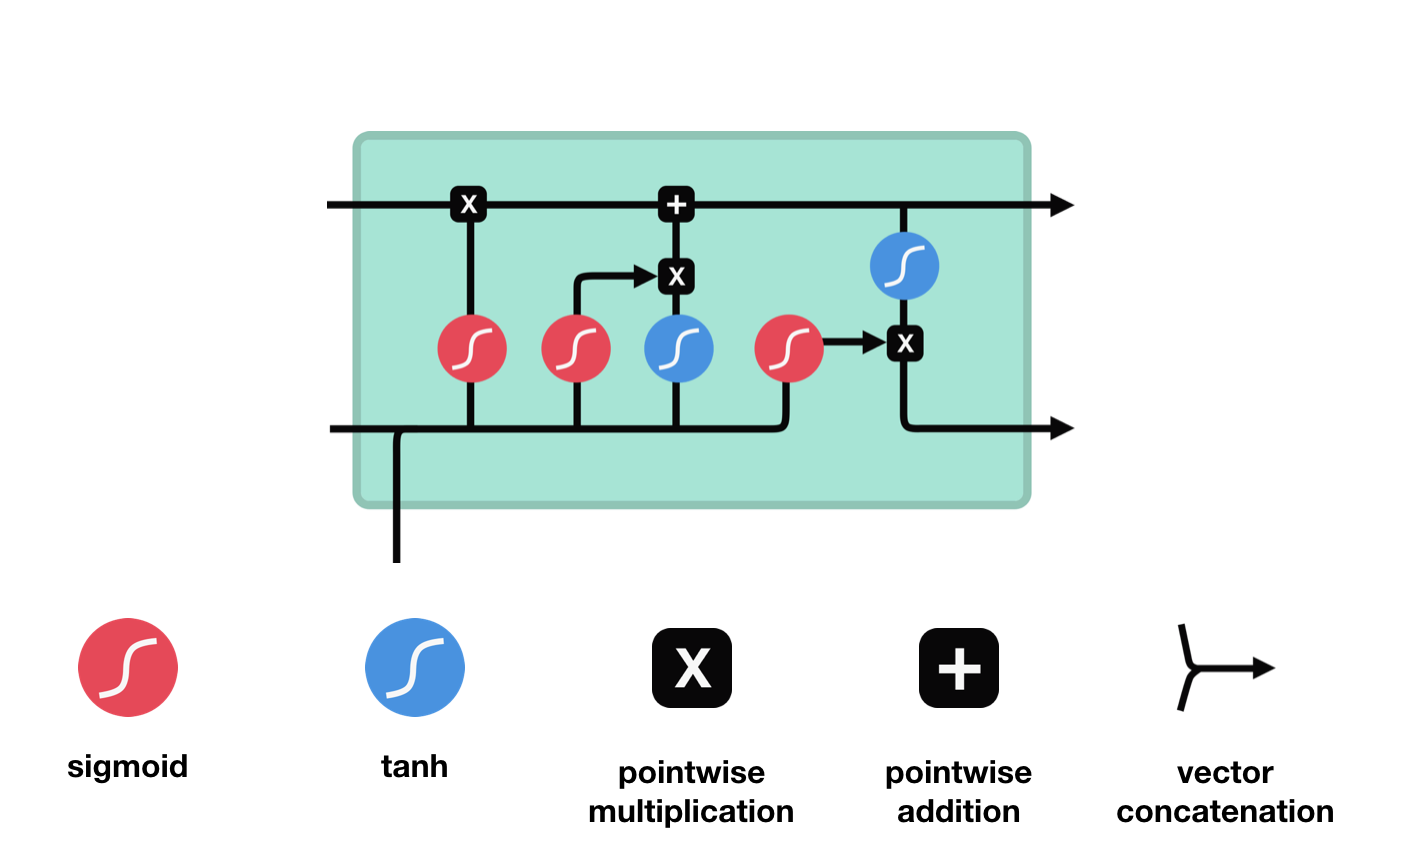
\includegraphics[width=0.85\textwidth]{../figures/diagrams/m4_rnn_architecture.png}
    \caption{RNN Architecture and LSTM cell structure from source material (Chapter 4 PPT), showing the unrolled recurrent network and the internal gating mechanisms of the LSTM cell.}
    \label{fig:m4_rnn_architecture}
\end{figure}

\subsection{Gated Recurrent Unit (GRU)}

The \textbf{Gated Recurrent Unit (GRU)}, introduced by Cho et al. in 2014, is a simplified variant of the LSTM that achieves similar performance with fewer parameters and faster training. The GRU merges the forget and input gates into a single \textbf{update gate} and eliminates the separate cell state, using only the hidden state to carry information across time steps.

The GRU has two gates:

\subsubsection{The Reset Gate}

The \textbf{reset gate} $r_t$ determines how much of the previous hidden state to forget when computing the candidate hidden state. If $r_t$ is close to 0, the past hidden state is largely ignored, and the candidate state depends mainly on the current input. If $r_t$ is close to 1, the past hidden state is fully preserved.
\[
r_t = \sigma(W_r \cdot [h_{t-1}, x_t])
\]

\subsubsection{The Update Gate}

The \textbf{update gate} $z_t$ determines how much of the previous hidden state to keep and how much of the new candidate hidden state to use. It is analogous to the combination of the forget and input gates in an LSTM.
\[
z_t = \sigma(W_z \cdot [h_{t-1}, x_t])
\]

The candidate hidden state is computed as:
\[
\tilde{h}_t = \tanh(W \cdot [r_t \odot h_{t-1}, x_t])
\]

And the final hidden state is a weighted combination of the old and candidate states:
\[
h_t = (1 - z_t) \odot h_{t-1} + z_t \odot \tilde{h}_t
\]

\begin{tcolorbox}[colback=blue!5!white,colframe=blue!75!black,title=\textbf{Key Insight: Interpreting the GRU Update Gate}]
The update gate $z_t$ controls the balance between old and new information:
\begin{itemize}
    \item \textbf{If $z_t \approx 0$}: Then $1 - z_t \approx 1$, so most of the old hidden state $h_{t-1}$ is preserved, and only a small amount of new information from $\tilde{h}_t$ is incorporated. This is useful when the current input is not very informative or when we want to maintain long-term memory.
    \item \textbf{If $z_t \approx 1$}: Then $1 - z_t \approx 0$, so the old hidden state is largely discarded, and the new candidate state $\tilde{h}_t$ dominates. This allows the network to rapidly update its memory when important new information arrives.
\end{itemize}
\end{tcolorbox}

\begin{figure}[H]
    \centering
    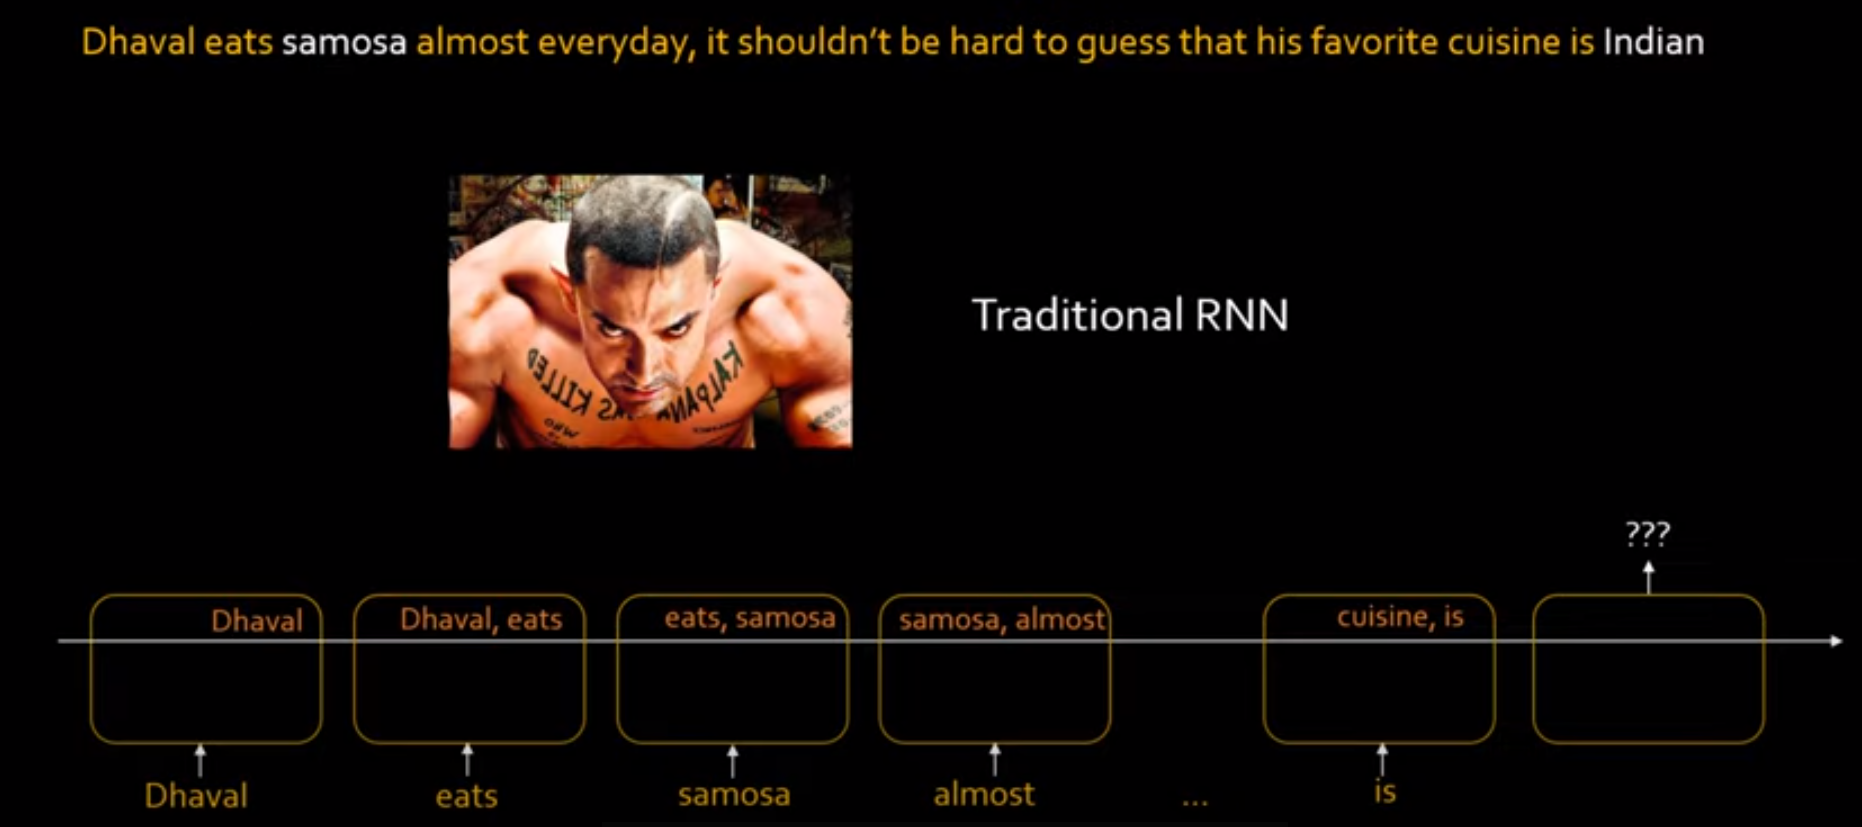
\includegraphics[width=0.85\textwidth]{../figures/diagrams/m4_gru_lstm.png}
    \caption{GRU and LSTM cell diagrams from source material (Gated Recurrent Unit PPT), comparing the internal structure and gating mechanisms of GRU and LSTM architectures.}
    \label{fig:m4_gru_lstm}
\end{figure}

\subsection{Bidirectional Recurrent Neural Networks (Bi-RNN)}

A standard RNN processes a sequence in one direction only---from left to right (or from past to future). This means that the prediction at time $t$ can only use information from positions $1, 2, \ldots, t$. For many tasks, however, it would be useful to also use information from the future context.

A \textbf{Bidirectional RNN (Bi-RNN)} addresses this limitation by processing the input sequence in \textbf{both directions simultaneously}. It consists of two separate hidden layers:
\begin{itemize}
    \item A \textbf{forward layer} that processes the sequence from left to right, computing hidden states $\overrightarrow{h}_1, \overrightarrow{h}_2, \ldots, \overrightarrow{h}_T$.
    \item A \textbf{backward layer} that processes the sequence from right to left, computing hidden states $\overleftarrow{h}_T, \overleftarrow{h}_{T-1}, \ldots, \overleftarrow{h}_1$.
\end{itemize}

The final representation at each time step is typically the concatenation of the forward and backward hidden states: $h_t = [\overrightarrow{h}_t; \overleftarrow{h}_t]$.

Bi-RNNs are particularly effective for tasks where the full context matters, such as:
\begin{itemize}
    \item \textbf{Sentiment analysis}: Words at the end of a sentence may change the sentiment of words at the beginning (e.g., ``The movie started slowly but ended brilliantly'').
    \item \textbf{Named entity recognition}: Determining whether ``Washington'' is a person or a location requires seeing the surrounding context on both sides.
    \item \textbf{Machine translation}: The meaning of a word in the source language may depend on words both before and after it.
\end{itemize}

\subsubsection{Advantages and Disadvantages of Bi-RNNs}

\textbf{Advantages}:
\begin{itemize}
    \item Access to both past and future context leads to more accurate predictions.
    \item Better handling of long-range dependencies because each layer only has to model half the sequence.
    \item The two layers provide a form of implicit regularization, reducing overfitting.
\end{itemize}

\textbf{Disadvantages}:
\begin{itemize}
    \item \textbf{Higher computational cost}: Two separate recurrent passes are required, roughly doubling computation time.
    \item \textbf{Longer training time}: More parameters and more computation mean slower training.
    \item \textbf{Difficulty in parallelization}: The sequential nature of both forward and backward passes makes parallelization challenging.
    \item \textbf{Cannot be used for real-time generation}: Because the backward pass requires seeing the entire sequence, Bi-RNNs cannot be used for tasks like real-time speech recognition or live text generation.
\end{itemize}

\begin{figure}[H]
    \centering
    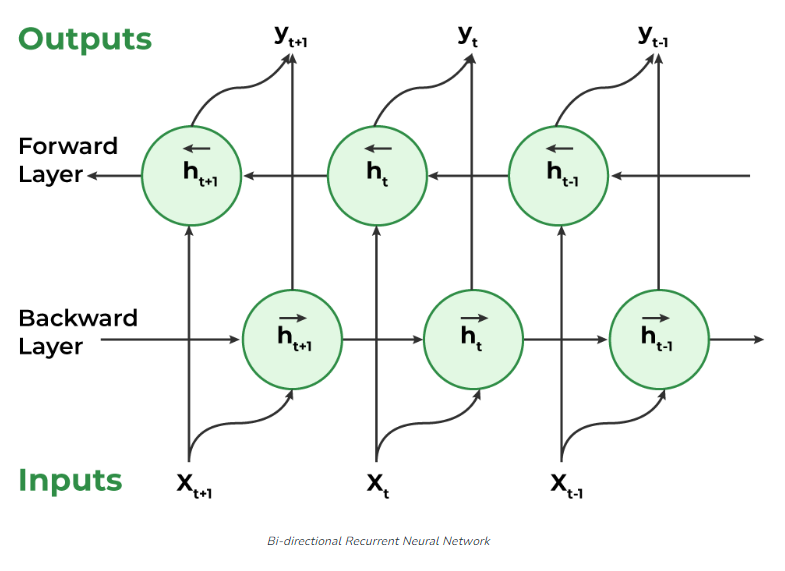
\includegraphics[width=0.75\textwidth]{../figures/diagrams/m4_bidirectional_rnn.png}
    \caption{Bidirectional RNN architecture from source material (Bidirectional RNN PPT), illustrating how forward and backward layers process the sequence in opposite directions and combine their outputs.}
    \label{fig:m4_bidirectional_rnn}
\end{figure}


\newpage

\section{Module 5: Morphology and Syntax}

\subsection{Morphology}

\textbf{Morphology} is the branch of linguistics that studies the internal structure of words and how words are formed from smaller meaningful units called morphemes. Understanding morphology is essential for many NLP tasks, including stemming, lemmatization, part-of-speech tagging, machine translation, and information retrieval, because it reveals the underlying structure and meaning of words that surface forms alone do not capture.

For example, the word ``uneducated'' can be broken down into three morphemes: ``un-'' (a prefix meaning ``not''), ``educate'' (the root or stem), and ``-d'' (a suffix indicating past participle). Similarly, the word ``playing'' consists of ``play'' (the stem) and ``-ing'' (a suffix indicating present participle). By decomposing words into their morphemic components, we can understand relationships between words, recognize inflected forms, and build more efficient vocabulary representations.

\subsubsection{Morphemes}

A \textbf{morpheme} is the smallest unit of language that carries meaning. Morphemes cannot be broken down into smaller meaningful parts. For example, the word ``cats'' contains two morphemes: ``cat'' (meaning a feline animal) and ``-s'' (meaning plural). Neither ``ca'' nor ``ts'' carries independent meaning.

The study of morphemes is fundamental because it explains how a finite set of morphemes can generate an infinite variety of words through systematic combination rules.

\subsubsection{Types of Morphemes}

Morphemes are broadly classified into two categories based on whether they can stand alone as words:

\begin{enumerate}
    \item \textbf{Free Morphemes}: These can appear as independent words and carry meaning on their own. Examples include ``house'', ``walk'', ``of'', and ``the''. When a free morpheme combines with bound morphemes, it is called the \textbf{stem} or \textbf{root} of the word.
    \item \textbf{Bound Morphemes}: These cannot stand alone as words; they must attach to free morphemes. Examples include ``-s'' (as in ``dogs''), ``-ly'' (as in ``quickly''), and ``un-'' (as in ``undo''). Bound morphemes are further divided into:
    \begin{itemize}
        \item \textbf{Prefixes}: Attach before the stem (e.g., ``un-'', ``re-'', ``pre-'')
        \item \textbf{Suffixes}: Attach after the stem (e.g., ``-ing'', ``-ed'', ``-s'')
        \item \textbf{Infixes}: Insert inside the stem (rare in English, common in some other languages)
    \end{itemize}
\end{enumerate}

\subsubsection{Lexical vs. Grammatical Morphemes}

Another important distinction is between lexical and grammatical morphemes:

\textbf{Lexical morphemes} (also called \textbf{content morphemes}) carry the core semantic content of a sentence. They belong to the ``open classes'' of a language---categories to which new words are regularly added. The major lexical categories are:
\begin{itemize}
    \item \textbf{Nouns}: Words referring to entities (e.g., ``dog'', ``happiness'', ``Google'')
    \item \textbf{Verbs}: Words referring to actions or states (e.g., ``run'', ``think'', ``Skype'')
    \item \textbf{Adjectives}: Words describing properties (e.g., ``red'', ``tall'')
    \item \textbf{Adverbs}: Words modifying verbs, adjectives, or other adverbs (e.g., ``quickly'', ``very'')
\end{itemize}

Because these are open classes, new words are constantly added to the language. Words like ``Google'', ``blog'', ``selfie'', and ``hashtag'' have all entered English in recent decades as new lexical morphemes.

\textbf{Grammatical morphemes} (also called \textbf{function morphemes}) belong to the ``closed classes''---categories with a fixed, limited membership that rarely admits new words. They serve to tie the content words together into coherent grammatical structures. Examples include:
\begin{itemize}
    \item \textbf{Conjunctions}: ``and'', ``but'', ``or'', ``because''
    \item \textbf{Prepositions}: ``in'', ``on'', ``at'', ``by'', ``with''
    \item \textbf{Articles}: ``the'', ``a'', ``an''
    \item \textbf{Pronouns}: ``I'', ``you'', ``he'', ``she'', ``it'', ``they''
\end{itemize}

\subsubsection{Inflectional vs. Derivational Morphology}

Morphemes can also be classified by the type of change they produce:

\textbf{Inflectional morphology} changes the grammatical form of a word without changing its word class (part of speech). English has only eight inflectional morphemes, all of which are suffixes:
\begin{itemize}
    \item \textbf{Plural}: ``-s'' / ``-es'' (cat $\to$ cats)
    \item \textbf{Possessive}: ``-'s'' (John $\to$ John's)
    \item \textbf{Third person singular present}: ``-s'' (walk $\to$ walks)
    \item \textbf{Past tense}: ``-ed'' (walk $\to$ walked)
    \item \textbf{Progressive}: ``-ing'' (walk $\to$ walking)
    \item \textbf{Past participle}: ``-ed'' / ``-en'' (eat $\to$ eaten)
    \item \textbf{Comparative}: ``-er'' (tall $\to$ taller)
    \item \textbf{Superlative}: ``-est'' (tall $\to$ tallest)
\end{itemize}

Inflections can be:
\begin{itemize}
    \item \textbf{Regular}: Follow standard, predictable patterns (walked, played, cats)
    \item \textbf{Irregular}: Do not follow standard patterns (go $\to$ went, child $\to$ children, wife $\to$ wives)
    \item \textbf{Suppletion}: Use a completely different morpheme (good $\to$ better, bad $\to$ worse, go $\to$ went)
\end{itemize}

\textbf{Derivational morphology} creates new words, often changing the word class:
\begin{itemize}
    \item \textbf{Class-changing}: care (verb) $\to$ careful (adjective) $\to$ carelessly (adverb)
    \item \textbf{Class-maintaining}: child (noun) $\to$ childhood (noun), friend (noun) $\to$ friendship (noun)
\end{itemize}

\begin{figure}[H]
    \centering
    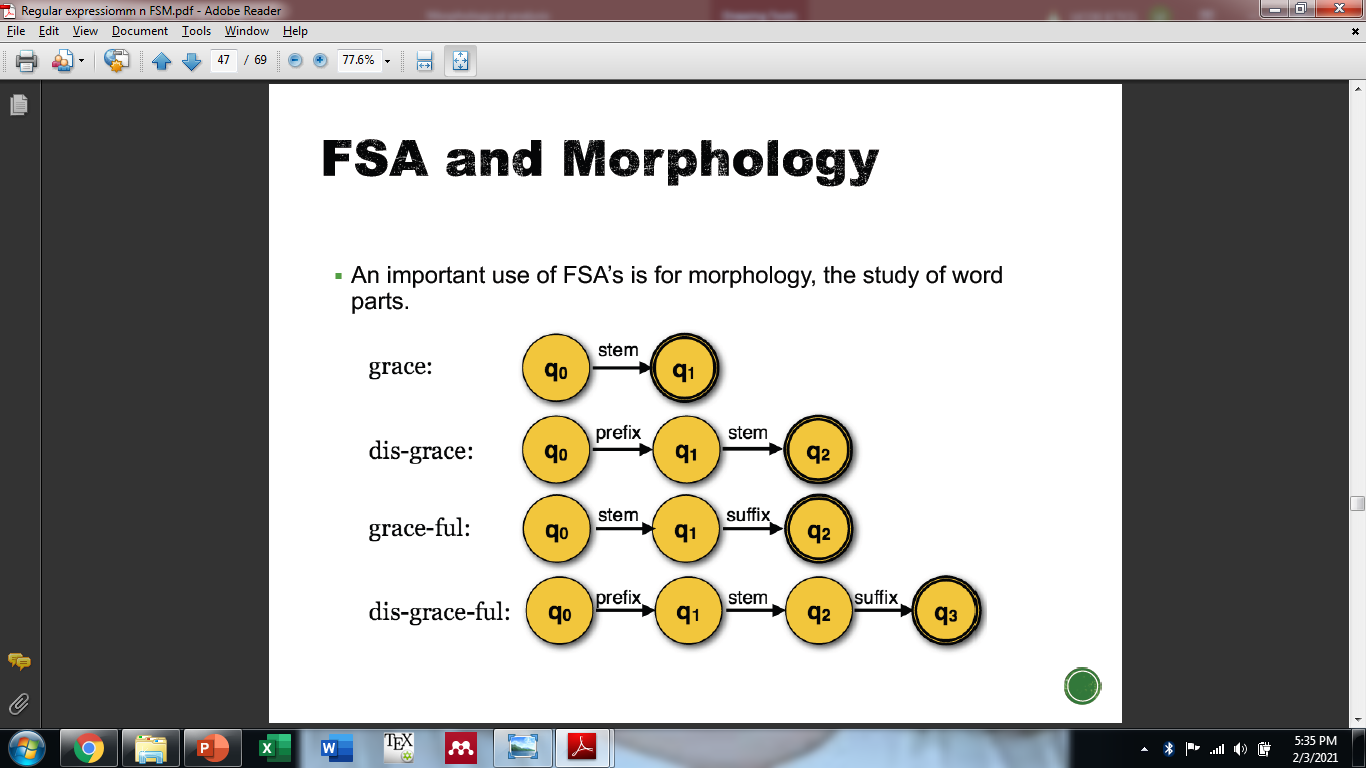
\includegraphics[width=0.85\textwidth]{../figures/diagrams/m5_morphology.png}
    \caption{Morphological Analysis framework from source material (Morphological Analysis PPT), illustrating the decomposition of words into morphemes and the relationships between morphological components.}
    \label{fig:m5_morphology}
\end{figure}

\subsection{Regular Expressions}

\textbf{Regular expressions} (often abbreviated as regex or regexp) are a formal language for specifying text search strings. They are one of the most fundamental tools in text processing and form the basis of many higher-level NLP techniques, including tokenization, pattern matching, and information extraction.

A regular expression is built from a small set of operators that can specify complex patterns concisely. The simplest regular expression is just a sequence of literal characters, which matches exactly that sequence. For example, the regular expression ``woodchuck'' matches the string ``woodchuck'' and nothing else.

\subsubsection{Disjunction}

\textbf{Disjunction} allows a regular expression to match alternative characters or sequences. The square brackets ``[ ]'' define a \textbf{character class} that matches any one of the enclosed characters. For example, ``[Ww]oodchuck'' matches both ``Woodchuck'' and ``woodchuck''.

Character classes can also specify \textbf{ranges}: ``[A-Z]'' matches any uppercase letter, ``[a-z]'' matches any lowercase letter, and ``[0-9]'' matches any digit.

The \textbf{negation operator} ``[\^{} ]'' inside a character class matches any character \textit{except} those listed. For example, ``[\^{}Ss]'' matches any character that is not ``S'' or ``s''.

The \textbf{pipe operator} ``|'' provides disjunction between full sequences rather than individual characters. For example, ``woodchuck|groundhog'' matches either ``woodchuck'' or ``groundhog''.

\subsubsection{Kleene Operators}

The \textbf{Kleene operators} allow regular expressions to specify repetition:
\begin{itemize}
    \item \textbf{Kleene * (star)}: Matches zero or more occurrences of the preceding element. ``ab*c'' matches ``ac'', ``abc'', ``abbc'', ``abbbc'', etc.
    \item \textbf{Kleene + (plus)}: Matches one or more occurrences. ``ab+c'' matches ``abc'', ``abbc'', etc., but not ``ac''.
    \item \textbf{? (question mark)}: Matches zero or one occurrence. ``colou?r'' matches both ``color'' and ``colour''.
    \item \textbf{. (dot)}: Matches any single character. ``a.c'' matches ``abc'', ``a1c'', ``a c'', etc.
\end{itemize}

\subsubsection{Anchors}

\textbf{Anchors} match positions in the text rather than characters:
\begin{itemize}
    \item \textbf{\^{}}: Matches the beginning of a line or string.
    \item \textbf{\$}: Matches the end of a line or string.
    \item \textbf{\textbackslash b}: Matches a word boundary (the position between a word character and a non-word character).
\end{itemize}

\subsubsection{Capture Groups and Backreferences}

\textbf{Capture groups} (parentheses ``( )'') group parts of a regular expression together and ``capture'' the matched substring for later use. \textbf{Backreferences} (``\textbackslash 1'', ``\textbackslash 2'', etc.) refer back to the captured groups. For example, the pattern ``s/([0-9]+)/<\textbackslash 1>/'' finds a sequence of digits and wraps it in angle brackets.

\subsubsection{Errors in Pattern Matching}

When designing regular expressions, two types of errors must be considered:
\begin{itemize}
    \item \textbf{False positives (Type I errors)}: The pattern matches strings that it should not match. This corresponds to low \textbf{precision}.
    \item \textbf{False negatives (Type II errors)}: The pattern fails to match strings that it should match. This corresponds to low \textbf{recall}.
\end{itemize}

A good regular expression balances precision and recall for the specific application.

\subsection{Finite State Automata}

A \textbf{Finite State Automaton (FSA)} (plural: automata) is the simplest abstract machine for recognizing patterns. It is an idealized model of a digital computer that has a finite number of states and transitions between those states based on input symbols.

Formally, an FSA is defined by five elements (a 5-tuple):
\begin{itemize}
    \item $Q$: A finite set of states
    \item $\Sigma$: A finite set of input symbols (the alphabet)
    \item $q_0 \in Q$: The initial (start) state
    \item $F \subseteq Q$: A set of final (accepting) states
    \item $\delta: Q \times \Sigma \to Q$: The transition function, which maps a state and an input symbol to a new state
\end{itemize}

An FSA processes an input string by starting in the initial state and following transitions according to each input symbol. If the automaton ends in a final state after reading the entire input, the string is \textbf{accepted}; otherwise, it is \textbf{rejected}.

\subsubsection{Deterministic Finite Automata (DFA)}

A \textbf{Deterministic Finite Automaton (DFA)} is a restricted form of FSA in which, for every state and every input symbol, there is exactly one possible next state. A DFA does not allow $\epsilon$-transitions (transitions that consume no input), and it does not allow multiple possible transitions for the same state-symbol pair.

DFAs are particularly important because every regular expression can be converted into an equivalent DFA, and DFAs can be efficiently implemented in software. The transition function of a DFA is a complete mapping $\delta: Q \times \Sigma \to Q$.

\subsection{Morphological Parsing}

\textbf{Morphological parsing} is the task of finding the lexical form (the underlying morpheme sequence) of a word from its surface form. For example, given the surface word ``cats'', a morphological parser should produce ``cat + N + PL'' (noun, plural). Given ``caught'', it should produce ``catch + V + PAST''.

A complete morphological parser requires three components:
\begin{enumerate}
    \item \textbf{Lexicon}: A repository of stems and affixes with their categories (noun, verb, adjective, etc.) and sub-categories (regular noun, irregular noun, etc.).
    \item \textbf{Morphotactics}: Rules specifying which classes of morphemes can follow which other classes. For example, in English, the plural morpheme (``-s'' or ``-es'') follows the stem but never precedes it.
    \item \textbf{Orthographic Rules}: Rules specifying spelling changes that occur when morphemes combine. For example, when ``care'' combines with ``-ing'', the ``e'' is dropped: ``caring'' (not ``careing''). When ``city'' combines with ``-es'', the ``y'' changes to ``i'': ``cities''.
\end{enumerate}

\subsubsection{Finite State Transducers (FST)}

A \textbf{Finite State Transducer (FST)} is a generalization of an FSA that operates on two (or more) tapes simultaneously. An FST reads from one tape and writes to another, making it ideal for morphological parsing where the input tape contains the surface form and the output tape contains the lexical form.

For example, an FST for English noun morphology might read ``cats'' from the input tape and write ``cat + N + PL'' to the output tape. FSTs for morphological parsing typically consist of multiple transducers running in parallel---one for the lexicon, one for the morphotactics, and one for each orthographic rule.

\subsubsection{Two-Level Morphology}

\textbf{Two-level morphology}, developed by Koskenniemi in 1983, represents the correspondence between the lexical level (abstract morpheme sequences) and the surface level (actual spelling). The mapping is implemented using FSTs, and orthographic rules are written in a special notation:
\[
a \Rightarrow b \ / \ c \_\_ \ d
\]
which reads: ``rewrite ``a'' as ``b'' when it occurs between ``c'' and ``d''.'' For example, the rule for English ``e''-deletion before ``-ing'' would be written as:
\[
e \Rightarrow \epsilon \ / \ \_\_ \ ing
\]
meaning ``delete ``e'' before ``ing''.''

\subsection{Stemming and Lemmatization}

\textbf{Stemming} and \textbf{lemmatization} are both techniques for reducing words to a canonical form, but they differ in their approach and output:

\textbf{Stemming} is a crude heuristic process that chops off the ends of words in the hope of achieving the root form. It does not use a vocabulary or morphological analysis---it simply applies a series of rules to strip suffixes. The resulting stem may not be a valid word. For example:
\begin{itemize}
    \item ``studies'' $\to$ ``studi''
    \item ``giving'' $\to$ ``giv''
    \item ``caring'' $\to$ ``car''
\end{itemize}

\textbf{Lemmatization} is more sophisticated: it uses a vocabulary and morphological analysis to reduce words to their dictionary form (lemma). The output is always a valid word. For example:
\begin{itemize}
    \item ``studies'' $\to$ ``study''
    \item ``giving'' $\to$ ``give''
    \item ``caring'' $\to$ ``care''
\end{itemize}

Both stemming and lemmatization are used to normalize text, reduce vocabulary size, and improve information retrieval by matching different inflected forms of the same word.

\subsection{The Porter Stemmer Algorithm}

The \textbf{Porter Stemmer}, developed by Martin Porter in 1980, is the most widely used stemming algorithm for English. It consists of five sets of suffix-stripping rules applied in sequence. Within each step, if more than one rule could apply to a word, the rule with the longest matching suffix is chosen.

\subsubsection{Measure of a Word}

Before applying the rules, the Porter Stemmer defines a ``measure'' $m$ of a word that captures its morphological complexity. A word is analyzed in terms of consonant (C) and vowel (V) sequences and has the general form:
\[
[C](VC)^m[V]
\]
where $[C]$ and $[V]$ are optional, and $m$ is the number of VC pairs. Examples:
\begin{itemize}
    \item $m = 0$: TR, EE, TREE, Y, BY
    \item $m = 1$: TROUBLE, OATS, TREES, IVY
    \item $m = 2$: TROUBLES, PRIVATE, OATEN, ORRERY
\end{itemize}

The condition ``$m > 1$'' in a rule means the stem must have a measure greater than 1, ensuring that very short stems are not over-stripped.

\subsubsection{Porter Stemmer Steps}

The algorithm proceeds through five steps:

\textbf{Step 1a}: Handles plurals and word forms ending in ``-s''.
\begin{center}
\begin{tabular}{|l|l|l|}
\hline
\textbf{Rule} & \textbf{Example} & \textbf{Result} \\ \hline
sses $\to$ ss & caresses & caress \\ \hline
ies $\to$ i & ponies & poni \\ \hline
ss $\to$ ss & caress & caress \\ \hline
s $\to$ $\emptyset$ & cats & cat \\ \hline
\end{tabular}
\end{center}

\textbf{Step 1b}: Handles past participles and gerunds.
\begin{center}
\begin{tabular}{|l|l|l|}
\hline
\textbf{Rule} & \textbf{Example} & \textbf{Result} \\ \hline
(m$>$0) eed $\to$ ee & agreed & agree \\ \hline
(*v*) ed $\to$ $\emptyset$ & plastered & plaster \\ \hline
(*v*) ing $\to$ $\emptyset$ & motoring & motor \\ \hline
\end{tabular}
\end{center}
If the second or third rule in Step 1b fires, a cleanup step applies additional rules (at $\to$ ate, bl $\to$ ble, iz $\to$ ize, etc.).

\textbf{Step 1c}: Y elimination.
\begin{itemize}
    \item (*v*) y $\to$ i: happy $\to$ happi, sky $\to$ ski (wait, no: sky remains sky because there is no vowel before y)
\end{itemize}

\textbf{Step 2}: Derivational morphology (m $>$ 0). A large set of rules strip common suffixes:
\begin{center}
\begin{tabular}{|l|l|l|}
\hline
\textbf{Rule} & \textbf{Example} & \textbf{Result} \\ \hline
ational $\to$ ate & relational & relate \\ \hline
tional $\to$ tion & conditional & condition \\ \hline
ization $\to$ ize & vietnamization & vietnamize \\ \hline
fulness $\to$ ful & hopefulness & hopeful \\ \hline
ness $\to$ $\emptyset$ & goodness & good \\ \hline
\end{tabular}
\end{center}

\textbf{Step 3}: More derivational suffixes (m $>$ 0).
\begin{center}
\begin{tabular}{|l|l|l|}
\hline
\textbf{Rule} & \textbf{Example} & \textbf{Result} \\ \hline
icate $\to$ ic & triplicate & triplic \\ \hline
ative $\to$ $\emptyset$ & formative & form \\ \hline
alize $\to$ al & formalize & formal \\ \hline
ness $\to$ $\emptyset$ & goodness & good \\ \hline
\end{tabular}
\end{center}

\textbf{Step 4}: Suffix removal (m $>$ 1). Removes a large set of suffixes including -al, -ance, -ence, -er, -ic, -able, -ible, -ant, -ement, -ment, -ent, -ism, -ate, -iti, -ous, -ive, -ize.

\textbf{Step 5a}: Final ``e'' removal (m $>$ 1 or m = 1 and not *o).
\begin{itemize}
    \item e $\to$ $\emptyset$: probate $\to$ probat, rate $\to$ rate (not removed because m=1 and *o applies)
\end{itemize}

\textbf{Step 5b}: Double ``l'' reduction (m $>$ 1 and *d and *L).
\begin{itemize}
    \item controll $\to$ control, roll $\to$ roll
\end{itemize}

\begin{figure}[H]
    \centering
    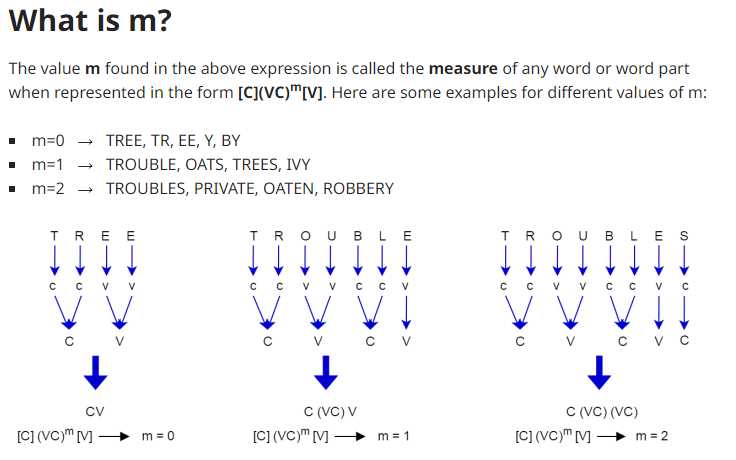
\includegraphics[width=0.65\textwidth]{../figures/diagrams/m5_porter_stemmer.png}
    \caption{Porter Stemmer Algorithm flow from source material (Porter Stemmer Algorithm PPT), illustrating the sequential rule application process and measure-based conditions.}
    \label{fig:m5_porter_stemmer}
\end{figure}

\subsection{Part-of-Speech (POS) Tagging}

\textbf{Part-of-Speech (POS) tagging} is the task of assigning a grammatical category---such as noun, verb, adjective, or adverb---to each word in a text. This is a fundamental preprocessing step for many NLP tasks because the grammatical role of a word provides crucial information for parsing, information extraction, and semantic analysis.

Words are often \textbf{ambiguous} with respect to part of speech. For example, ``book'' can be a noun (``hand me that book'') or a verb (``book that flight''). The goal of POS tagging is to resolve these ambiguities by choosing the proper tag for the context.

\subsubsection{POS Tag Sets}

Different applications require different levels of granularity in POS tagging:
\begin{itemize}
    \item \textbf{Coarse-grained tag sets} use a small number of general categories (e.g., just ``Noun'', ``Verb'', ``Adjective''). These are suitable for applications where fine grammatical distinctions are not needed.
    \item \textbf{Fine-grained tag sets} provide detailed grammatical information, including number (singular/plural), tense (past/present/future), and case. Common fine-grained tag sets include:
    \begin{itemize}
        \item \textbf{Penn Treebank}: 45 tags
        \item \textbf{Brown Corpus}: 87 tags
        \item \textbf{C7 tag set}: 146 tags
    \end{itemize}
\end{itemize}

The nine traditional word classes are: noun, verb, adjective, adverb, preposition, pronoun, determiner, conjunction, and interjection.

\subsubsection{POS Tagging Approaches}

Three major families of POS tagging algorithms have been developed:
\begin{enumerate}
    \item \textbf{Rule-based tagging}: Uses hand-crafted rules and a dictionary of possible tags for each word. In the first stage, all possible tags are assigned to each word. In the second stage, hand-written disambiguation rules remove incorrect tags until each word has exactly one tag. Early rule-based taggers like TAGGIT used 71 tags and 3,300 rules, achieving 77\% accuracy on the Brown Corpus.
    \item \textbf{Stochastic (probabilistic) tagging}: Uses statistical models, typically Hidden Markov Models (HMMs), to assign the most probable tag sequence given the observed word sequence. This is the most common approach and achieves very high accuracy (over 97\% on standard corpora).
    \item \textbf{Transformation-based tagging}: Uses learned rules (e.g., the Brill tagger) that iteratively correct errors made by an initial tagger. Rules are learned from a tagged training corpus.
\end{enumerate}

\begin{figure}[H]
    \centering
    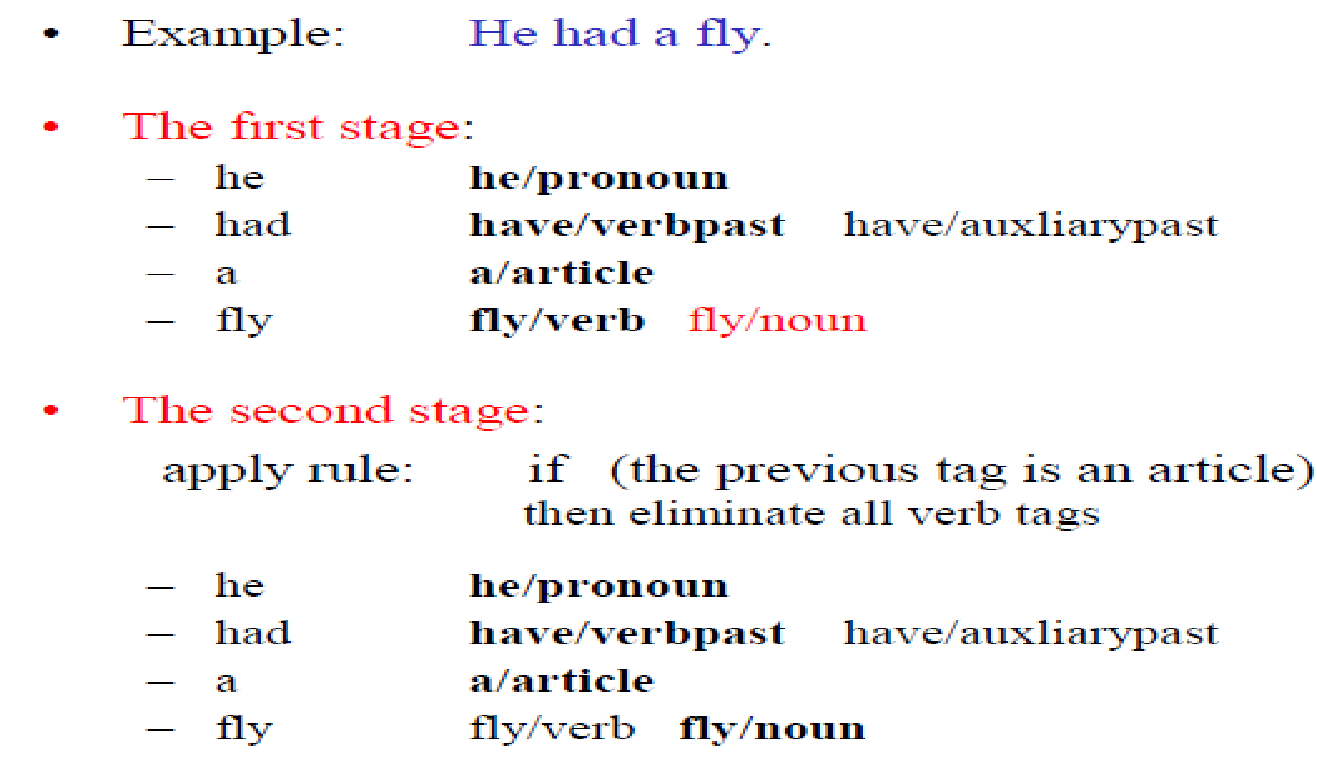
\includegraphics[width=0.85\textwidth]{../figures/diagrams/m5_pos_tagging.png}
    \caption{Part-of-Speech Tagging pipeline and HMM-based tagging approach from source material (Syntax Analysis PPT), showing the transition from raw text to tagged output.}
    \label{fig:m5_pos_tagging}
\end{figure}

\subsection{Hidden Markov Model (HMM) for POS Tagging}

The \textbf{Hidden Markov Model (HMM)} is the most widely used statistical model for POS tagging. An HMM is a probabilistic sequence model that computes a probability distribution over possible tag sequences and chooses the best one.

An HMM for POS tagging makes two key simplifying assumptions:
\begin{enumerate}
    \item \textbf{Markov assumption}: The probability of a tag depends only on the previous tag, not on the entire tag history. This is the bigram tag assumption: $P(t_i \mid t_1, \ldots, t_{i-1}) \approx P(t_i \mid t_{i-1})$.
    \item \textbf{Output independence}: The probability of a word depends only on its own tag, not on neighboring words or tags: $P(w_i \mid t_1, \ldots, t_n) \approx P(w_i \mid t_i)$.
\end{enumerate}

\subsubsection{HMM Components}

An HMM tagger has two probability matrices:

\textbf{The A matrix (transition probabilities)}: $P(t_i \mid t_{i-1})$ represents the probability of a tag occurring given the previous tag. For example, modal verbs like ``will'' are very likely to be followed by a base-form verb (VB). The MLE estimate is:
\[
P(t_i \mid t_{i-1}) = \frac{C(t_{i-1}, t_i)}{C(t_{i-1})}
\]

\textbf{The B matrix (emission probabilities)}: $P(w_i \mid t_i)$ represents the probability that a word $w_i$ is generated by tag $t_i$. For example, the word ``the'' is very likely to have the tag ``DET'' (determiner). The MLE estimate is:
\[
P(w_i \mid t_i) = \frac{C(w_i, t_i)}{C(t_i)}
\]

\subsubsection{HMM Decoding}

The goal of HMM decoding (also called \textbf{tagging}) is to find the most probable tag sequence $t_1, t_2, \ldots, t_n$ given the observed word sequence $w_1, w_2, \ldots, w_n$:
\[
\hat{t} = \arg\max_t P(t \mid w) = \arg\max_t \frac{P(w \mid t) P(t)}{P(w)} \approx \arg\max_t P(w \mid t) P(t)
\]

Because the denominator $P(w)$ is the same for all tag sequences, we only need to maximize the numerator.

\subsection{The Viterbi Algorithm}

The \textbf{Viterbi algorithm} is a dynamic programming algorithm for finding the most probable sequence of hidden states (tags) in an HMM. It is exponentially more efficient than brute-force enumeration because it exploits the Markov property to avoid recomputing probabilities for partial paths.

The key insight of the Viterbi algorithm is that the most probable path to any state at time $t$ must extend the most probable path to some state at time $t-1$. Therefore, for each possible tag at each position, we only need to keep track of the single best path that leads to it.

The algorithm proceeds as follows:
\begin{enumerate}
    \item \textbf{Initialization}: For each possible initial tag, compute the probability of starting with that tag and emitting the first word.
    \item \textbf{Recursion}: For each subsequent word, and for each possible tag, compute the probability of the best path to that tag by considering all possible previous tags and choosing the one that gives the maximum probability.
    \item \textbf{Termination}: After processing all words, choose the final tag with the highest probability.
    \item \textbf{Backtracking}: Trace back through the stored pointers to reconstruct the complete tag sequence.
\end{enumerate}

The time complexity of the Viterbi algorithm is $O(T \cdot N^2)$, where $T$ is the sentence length and $N$ is the number of possible tags. This is dramatically better than the $O(N^T)$ complexity of brute-force enumeration.

\begin{tcolorbox}[colback=green!5!white,colframe=green!75!black,title=\textbf{Numerical: HMM Tagging with Viterbi}]
\textbf{Sentence}: ``Will can spot Mary''

Possible tags for each word: ``Will'' (MD/modal, NN/noun, VB/verb), ``can'' (MD/modal, NN/noun, VB/verb), ``spot'' (NN/noun, VB/verb), ``Mary'' (NNP/proper noun).

The Viterbi algorithm computes cumulative path probabilities:
\begin{enumerate}
    \item At position 1 (``Will''), compute $P(\text{tag}) \times P(\text{Will} \mid \text{tag})$ for each possible tag.
    \item At position 2 (``can''), for each possible tag, compute the best path probability by maximizing over all previous tags: $P(\text{tag}_2 \mid \text{tag}_1) \times P(\text{can} \mid \text{tag}_2) \times v_1(\text{tag}_1)$.
    \item Repeat for positions 3 and 4.
    \item At position 4, choose the tag with the highest probability and trace back to find the optimal path.
\end{enumerate}

The optimal path depends on the specific transition and emission probabilities from the training corpus, but the Viterbi algorithm guarantees finding the globally most probable tag sequence under the HMM assumptions.
\end{tcolorbox}

\subsection{Context-Free Grammars (CFG)}

A \textbf{Context-Free Grammar (CFG)} is a formal system for modeling the constituent structure of sentences in natural language (and programming languages). CFGs are the backbone of many syntactic formalisms and computational applications including grammar checking, semantic interpretation, dialogue understanding, and machine translation.

A CFG consists of:
\begin{itemize}
    \item A set of \textbf{production rules} that specify how symbols can be rewritten into sequences of other symbols
    \item A \textbf{lexicon} of terminal symbols (words)
\end{itemize}

The symbols in a CFG are divided into two classes:
\begin{itemize}
    \item \textbf{Terminal symbols}: Words that actually appear in the language (e.g., ``the'', ``flight'')
    \item \textbf{Non-terminal symbols}: Abstract categories that represent groups of terminals or other non-terminals (e.g., NP for noun phrase, VP for verb phrase, S for sentence)
\end{itemize}

Every CFG has a \textbf{start symbol} (usually S), and the set of all strings derivable from the start symbol constitutes the language defined by the grammar.

\subsubsection{Example CFG Rules}

A simple CFG for English air travel queries might include:
\begin{center}
\begin{tabular}{|l|l|}
\hline
\textbf{Rule} & \textbf{Example Derivation} \\ \hline
S $\to$ NP VP & ``I prefer a morning flight'' \\ \hline
NP $\to$ Det Noun & ``a flight'' \\ \hline
VP $\to$ Verb NP & ``prefer a morning flight'' \\ \hline
VP $\to$ Verb NP PP & ``leave Boston in the morning'' \\ \hline
VP $\to$ Verb PP & ``leaving on Thursday'' \\ \hline
PP $\to$ Preposition NP & ``from Los Angeles'' \\ \hline
\end{tabular}
\end{center}

\subsubsection{Syntactic Ambiguity}

A major challenge in parsing with CFGs is \textbf{ambiguity}: a single sentence may have multiple valid parse trees. Two common types of ambiguity are:
\begin{itemize}
    \item \textbf{Attachment ambiguity}: A constituent can attach at more than one place in the tree. For example, in ``We saw the Eiffel Tower flying to Paris'', the phrase ``flying to Paris'' could modify ``We'' (we were flying) or ``the Eiffel Tower'' (the tower was flying).
    \item \textbf{Coordination ambiguity}: Phrases conjoined by ``and'' can be grouped in multiple ways. For example, ``old men and women'' could mean [old [men and women]] (all are old) or [[old men] and [women]] (only the men are old).
\end{itemize}

\begin{figure}[H]
    \centering
    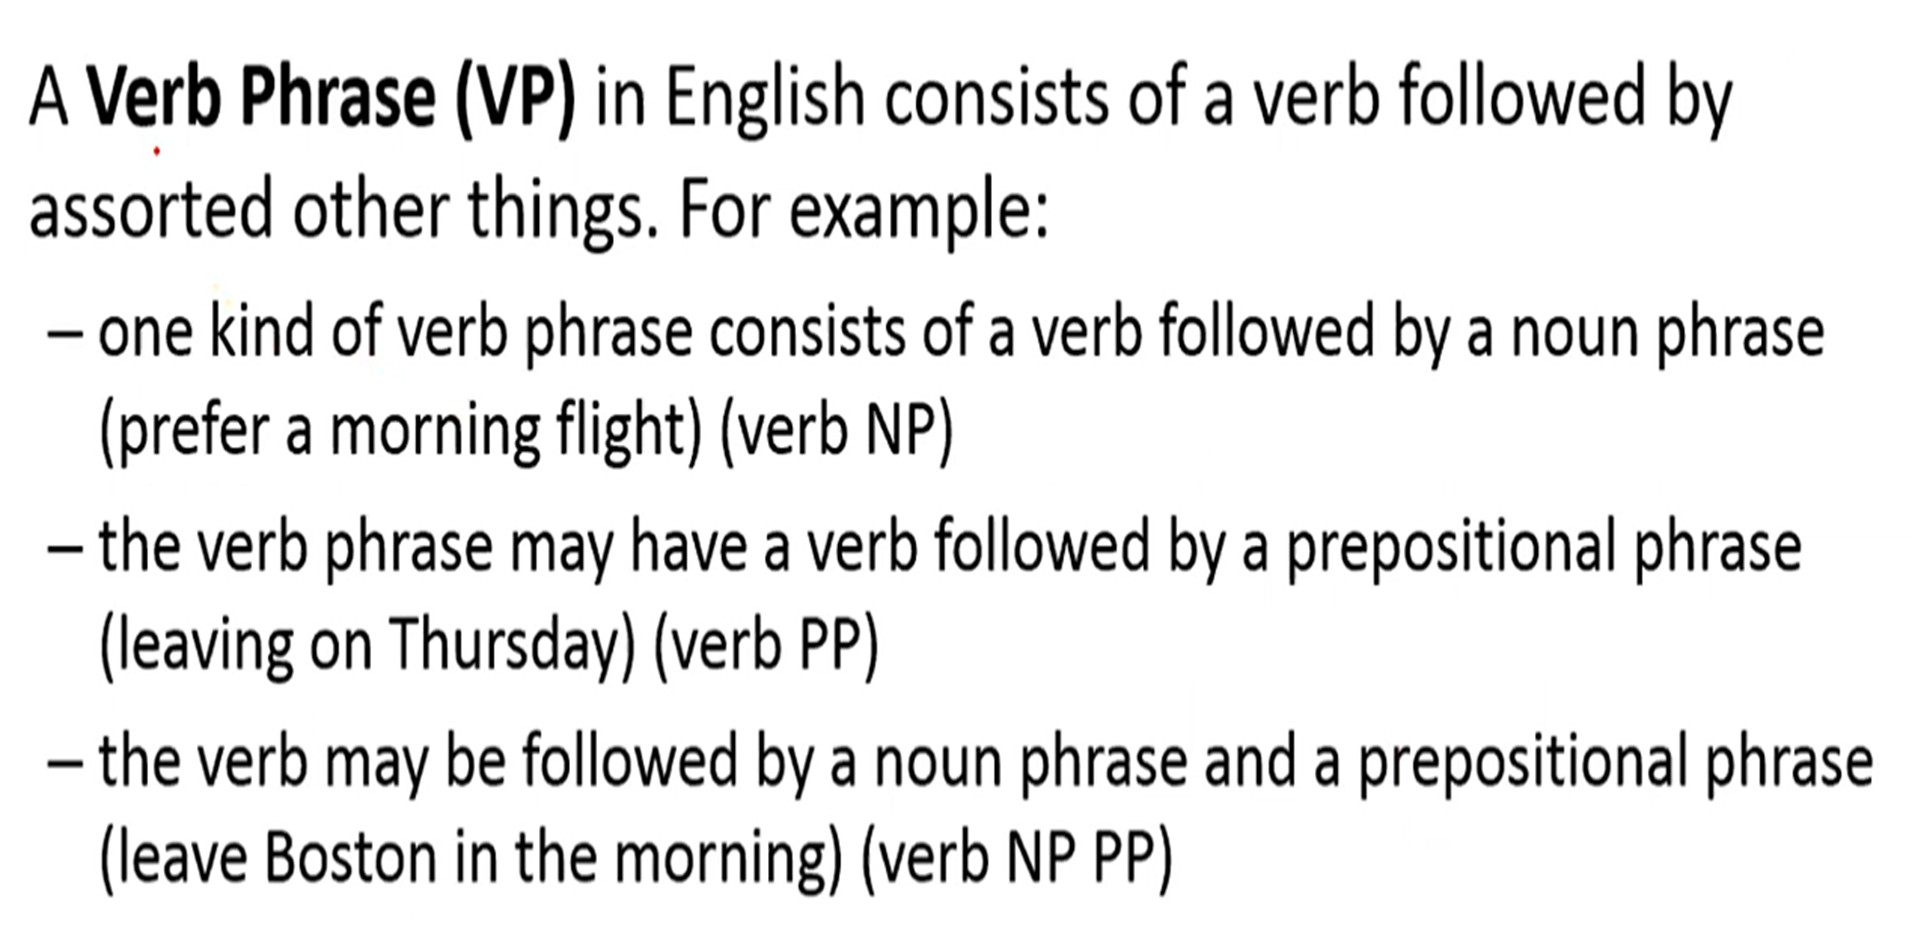
\includegraphics[width=0.85\textwidth]{../figures/diagrams/m5_cfg_parsing.png}
    \caption{Constituency Grammar and Parse Tree examples from source material (Constituency Grammars PPT), showing how CFG rules generate hierarchical syntactic structures.}
    \label{fig:m5_cfg_parsing}
\end{figure}

\subsection{CKY Parsing Algorithm}

The \textbf{Cocke-Younger-Kasami (CKY)} algorithm is a dynamic programming algorithm for parsing with CFGs. It determines whether a sentence can be generated by a grammar and, if so, finds one or all parse trees.

The CKY algorithm requires the grammar to be in \textbf{Chomsky Normal Form (CNF)}, where every production rule is either:
\begin{itemize}
    \item $A \to B \ C$ (two non-terminals on the right-hand side), or
    \item $A \to a$ (a single terminal on the right-hand side)
\end{itemize}

Any CFG can be systematically converted to CNF by introducing new non-terminals and splitting rules.

The algorithm constructs a table $T$ of size $N \times N$ for a sentence of length $N$, where $T[i, j]$ contains all non-terminals that can derive the substring from position $i$ to $j$. The table is filled from left to right and bottom to top:
\begin{enumerate}
    \item \textbf{Base case}: For each word at position $i$, find all non-terminals that can directly generate that word and add them to $T[i, i]$.
    \item \textbf{Inductive step}: For each substring of length $> 1$, try all possible ways to split the substring into two parts and check if any grammar rule combines a non-terminal from the left part with a non-terminal from the right part.
\end{enumerate}

The sentence is grammatical if and only if the start symbol $S$ appears in $T[1, N]$.

The time complexity of CKY is $O(N^3 \cdot |G|)$, where $N$ is the sentence length and $|G|$ is the grammar size. This is efficient enough for most practical parsing tasks.

\subsection{Probabilistic Context-Free Grammar (PCFG)}

A \textbf{Probabilistic Context-Free Grammar (PCFG)} extends a CFG by assigning a probability to each production rule. The probability of a parse tree is the product of the probabilities of all rules used in its derivation.

PCFGs address the ambiguity problem by choosing the most probable parse tree among all valid parses of a sentence. If multiple parse trees are possible, the one with the highest probability (according to the grammar) is selected as the correct analysis.

For example, if the grammar assigns higher probability to the rule ``NP $\to$ Adj NP'' than to ``NP $\to$ NP conj NP'', it will prefer the interpretation where ``old'' modifies the entire conjoined noun phrase rather than just ``men''.

The rule probabilities are typically estimated from a treebank (a corpus of sentences annotated with parse trees) using Maximum Likelihood Estimation:
\[
P(\alpha \to \beta \mid \alpha) = \frac{C(\alpha \to \beta)}{C(\alpha)}
\]
where $C(\alpha \to \beta)$ is the count of times the rule was seen in the treebank.

\begin{figure}[H]
    \centering
    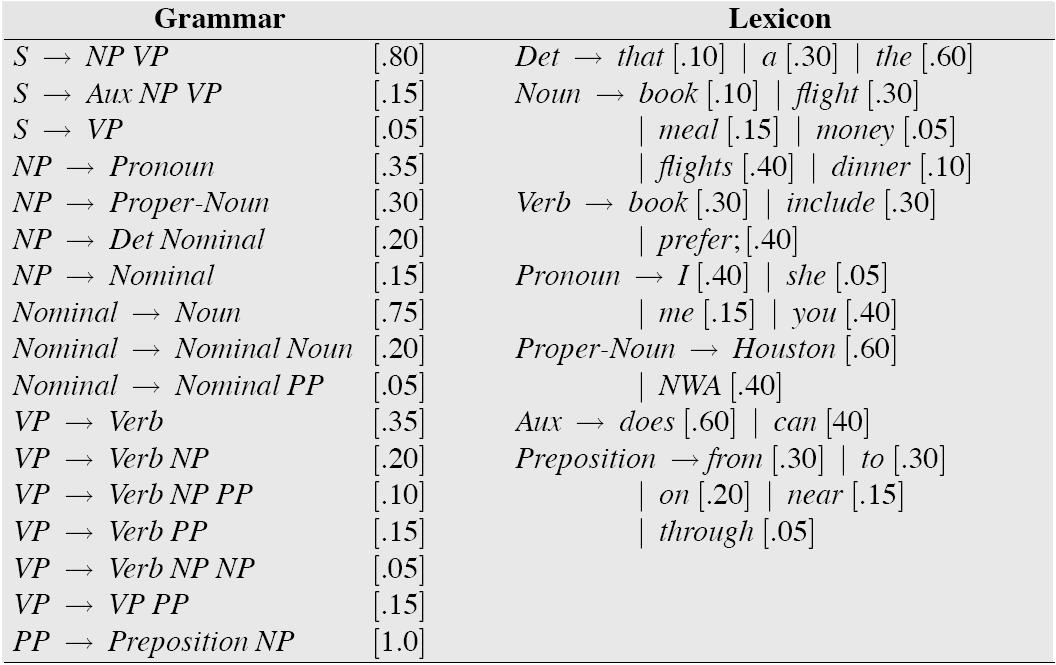
\includegraphics[width=0.75\textwidth]{../figures/diagrams/m5_pcfg.jpg}
    \caption{Probabilistic Context-Free Grammar and parse tree probabilities from source material (PCFG PPT), showing how rule probabilities resolve syntactic ambiguities.}
    \label{fig:m5_pcfg}
\end{figure}

\subsection{Dependency Parsing}

\textbf{Dependency parsing} is an alternative to constituency parsing (CFG-based parsing) that focuses on the \textbf{dependency relationships} between words rather than the hierarchical phrase structure. In a dependency parse, each word in the sentence is linked to exactly one other word (its \textbf{head} or \textbf{governor}) via a directed edge labeled with a grammatical relation (e.g., subject, object, modifier).

Dependency parsing is particularly valuable for languages with \textbf{free word order}, where the same meaning can be expressed with different word arrangements. For example, ``Boy handsome'' and ``Handsome boy'' might both be valid in some languages, and a dependency parser would recognize that ``boy'' is the head and ``handsome'' is its modifier in both cases, regardless of surface order.

\subsubsection{Key Terminology}

\begin{itemize}
    \item \textbf{Head (Governor)}: The word that dominates the relationship. In the pair (book, me), ``book'' is the head.
    \item \textbf{Dependent}: The word that is subordinate to the head. In (book, me), ``me'' is the dependent.
    \item \textbf{Root}: The single word in the sentence that has no head (it is the top of the dependency tree). Every sentence has exactly one root.
    \item \textbf{Arc}: The directed edge from head to dependent, labeled with a grammatical function (e.g., nsubj for nominal subject, obj for direct object, iobj for indirect object).
\end{itemize}

\subsubsection{Properties of Dependency Trees}

A well-formed dependency tree must satisfy three properties:
\begin{enumerate}
    \item The root has no incoming arcs.
    \item Every vertex (except the root) has exactly one incoming arc.
    \item There is a unique path from the root to each vertex.
\end{enumerate}

These properties ensure that the dependency structure is a directed tree (or arborescence) rooted at the main verb or predicate of the sentence.

\subsubsection{Projectivity}

A dependency tree is \textbf{projective} if, for every arc from head $h$ to dependent $d$, all words between $h$ and $d$ in the linear order of the sentence are descendants of $h$. In other words, no crossing edges exist. Projective trees correspond to the notion of nested constituents and can be parsed efficiently. Non-projective trees (with crossing edges) occur in some languages with more flexible word order.

\subsubsection{Shift-Reduce Parsing (Arc Standard)}

\textbf{Shift-reduce parsing} is a widely used algorithm for dependency parsing. It uses three data structures:
\begin{itemize}
    \item A \textbf{stack} (initially containing only a ROOT symbol)
    \item A \textbf{buffer} of input words (initially containing all words of the sentence in order)
    \item A set of \textbf{dependency relations} (initially empty)
\end{itemize}

The parser performs three types of transitions:
\begin{enumerate}
    \item \textbf{SHIFT}: Remove the first word from the buffer and push it onto the stack.
    \item \textbf{LEFTARC}: Pop the top two elements from the stack. Create a dependency relation from the second element to the first (the second is the head, the first is the dependent). Push the second element back onto the stack.
    \item \textbf{RIGHTARC}: Pop the top two elements from the stack. Create a dependency relation from the second element to the first (the second is the head, the first is the dependent). Push the first element back onto the stack.
\end{enumerate}

Parsing terminates when the buffer is empty and the stack contains only the ROOT symbol. The sequence of LEFTARC and RIGHTARC transitions defines the complete dependency tree.

\begin{tcolorbox}[colback=green!5!white,colframe=green!75!black,title=\textbf{Numerical: Dependency Parsing Example}]
\textbf{Sentence}: ``book me the morning flight''

\textbf{Step 0}: Stack = [ROOT], Buffer = [book, me, the, morning, flight]

\textbf{Step 1}: SHIFT $\to$ Stack = [ROOT, book]

\textbf{Step 2}: SHIFT $\to$ Stack = [ROOT, book, me]

\textbf{Step 3}: RIGHTARC(book, me) $\to$ Stack = [ROOT, book], Relations: book $\to$ me

\textbf{Step 4}: SHIFT $\to$ Stack = [ROOT, book, the]

\textbf{Step 5}: SHIFT $\to$ Stack = [ROOT, book, the, morning]

\textbf{Step 6}: SHIFT $\to$ Stack = [ROOT, book, the, morning, flight]

\textbf{Step 7}: LEFTARC(the, flight) $\to$ Stack = [ROOT, book, the, flight]

\textbf{Step 8}: LEFTARC(morning, flight) $\to$ Stack = [ROOT, book, flight]

\textbf{Step 9}: LEFTARC(book, flight) $\to$ Stack = [ROOT, book]

\textbf{Step 10}: RIGHTARC(ROOT, book) $\to$ Stack = [ROOT]

\textbf{Final dependency tree}:
\begin{itemize}
    \item ROOT $\to$ book (root relation)
    \item book $\to$ me (direct object)
    \item book $\to$ flight (indirect object / nominal complement)
    \item flight $\to$ the (determiner)
    \item flight $\to$ morning (modifier)
\end{itemize}
\end{tcolorbox}

\begin{figure}[H]
    \centering
    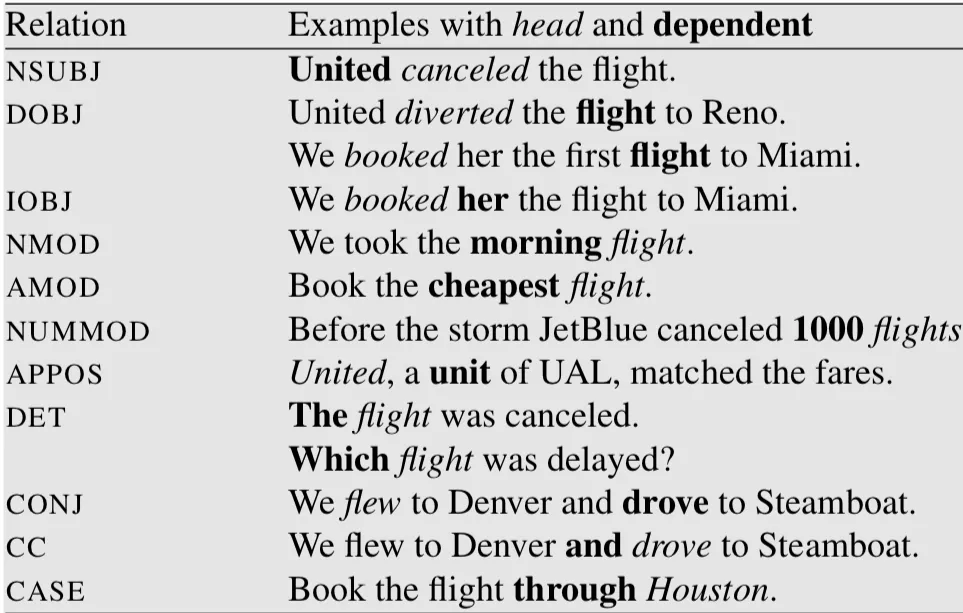
\includegraphics[width=0.85\textwidth]{../figures/diagrams/m5_dependency.png}
    \caption{Dependency Parsing visualization from source material (Dependency Parsing PPT), showing the dependency relations and arcs for a sample sentence with labeled grammatical functions.}
    \label{fig:m5_dependency}
\end{figure}


\newpage

\section{Summary of Key Concepts by Module}

\subsection{Module 1: N-gram Language Models and Edit Distance}
\begin{itemize}
    \item \textbf{Language models} assign probabilities to word sequences and predict upcoming words.
    \item \textbf{N-grams} model sequences of $n$ words; bigrams and trigrams are most common.
    \item \textbf{MLE} estimates probabilities from training corpus counts: $P(w_n \mid w_{n-1}) = C(w_{n-1}, w_n) / C(w_{n-1})$.
    \item \textbf{Perplexity} measures model quality: $\text{PP}(W) = P(W)^{-1/N}$. Lower is better.
    \item \textbf{Smoothing} (Laplace, add-k, interpolation, stupid backoff) handles unseen n-grams.
    \item \textbf{Entropy} and \textbf{cross-entropy} provide information-theoretic foundations for perplexity.
    \item \textbf{Edit distance} measures string similarity via minimum insertion, deletion, and substitution operations.
\end{itemize}

\subsection{Module 2: Word Senses, WordNet, and Vector Semantics}
\begin{itemize}
    \item \textbf{Word senses} are discrete meaning representations; polysemy and homonymy describe multiple senses.
    \item \textbf{Lexical relations}: synonymy, antonymy, hyponymy, hypernymy, meronymy.
    \item \textbf{WordNet} is a large lexical database organizing words into synsets with glosses and sense relations.
    \item \textbf{WSD} selects the correct sense in context; best modern approach uses contextual embeddings (BERT).
    \item \textbf{PMI/PPMI} measures word co-occurrence association: $\text{PMI}(w, c) = \log_2 \frac{P(w, c)}{P(w)P(c)}$.
    \item \textbf{Word Sense Induction} discovers senses automatically via clustering of context vectors.
\end{itemize}

\subsection{Module 3: Naive Bayes and Text Classification}
\begin{itemize}
    \item \textbf{Text classification} assigns labels to documents; applications include sentiment analysis and spam detection.
    \item \textbf{Naive Bayes} is a generative classifier using Bayes' rule with conditional independence and bag-of-words assumptions.
    \item \textbf{Training}: Estimate $P(c)$ and $P(w \mid c)$ with MLE + Laplace (add-1) smoothing.
    \item \textbf{Optimizations}: Binary multinomial NB, negation handling, sentiment lexicons.
\end{itemize}

\subsection{Module 4: Deep Learning for Sequences}
\begin{itemize}
    \item \textbf{RNNs} process sequences via hidden state recurrence: $h_t = \tanh(W_h h_{t-1} + W_x x_t + b_h)$.
    \item \textbf{BPTT} trains RNNs by unrolling through time and backpropagating gradients.
    \item \textbf{Vanishing/exploding gradients} limit RNNs' ability to learn long-range dependencies.
    \item \textbf{LSTM} solves this via cell state and forget/input/output gates.
    \item \textbf{GRU} simplifies LSTM with reset and update gates, using only the hidden state.
    \item \textbf{Bi-RNNs} process sequences in both directions, using full context but doubling computation.
\end{itemize}

\subsection{Module 5: Morphology and Syntax}
\begin{itemize}
    \item \textbf{Morphology} studies word structure; morphemes are the smallest meaning-bearing units (free vs. bound, lexical vs. grammatical, inflectional vs. derivational).
    \item \textbf{Regular expressions} use disjunction, Kleene operators, anchors, and capture groups for pattern matching.
    \item \textbf{FSA/DFA} recognize patterns via state transitions; 5-tuple formalism.
    \item \textbf{Porter Stemmer} applies 5 sequential steps with measure-based conditions to strip suffixes.
    \item \textbf{POS tagging} assigns grammatical categories; approaches include rule-based, HMM, and transformation-based.
    \item \textbf{HMM} uses transition and emission probabilities; Viterbi algorithm finds the optimal tag sequence.
    \item \textbf{CFG} defines syntactic structure via production rules with terminals and non-terminals.
    \item \textbf{CKY} parses CFGs in CNF using dynamic programming ($O(N^3)$).
    \item \textbf{PCFG} adds probabilities to CFG rules for disambiguation.
    \item \textbf{Dependency parsing} uses shift-reduce with LEFTARC/RIGHTARC/SHIFT to build head-dependent trees.
\end{itemize}

\end{document}
